\documentclass[twoside]{book}

% Packages required by doxygen
\usepackage{calc}
\usepackage{doxygen}
\usepackage{graphicx}
\usepackage[utf8]{inputenc}
\usepackage{makeidx}
\usepackage{multicol}
\usepackage{multirow}
\usepackage{textcomp}
\usepackage[table]{xcolor}

% Font selection
\usepackage[T1]{fontenc}
\usepackage{mathptmx}
\usepackage[scaled=.90]{helvet}
\usepackage{courier}
\usepackage{amssymb}
\usepackage{sectsty}
\renewcommand{\familydefault}{\sfdefault}
\allsectionsfont{%
  \fontseries{bc}\selectfont%
  \color{darkgray}%
}
\renewcommand{\DoxyLabelFont}{%
  \fontseries{bc}\selectfont%
  \color{darkgray}%
}

% Page & text layout
\usepackage{geometry}
\geometry{%
  a4paper,%
  top=2.5cm,%
  bottom=2.5cm,%
  left=2.5cm,%
  right=2.5cm%
}
\tolerance=750
\hfuzz=15pt
\hbadness=750
\setlength{\emergencystretch}{15pt}
\setlength{\parindent}{0cm}
\setlength{\parskip}{0.2cm}
\makeatletter
\renewcommand{\paragraph}{%
  \@startsection{paragraph}{4}{0ex}{-1.0ex}{1.0ex}{%
    \normalfont\normalsize\bfseries\SS@parafont%
  }%
}
\renewcommand{\subparagraph}{%
  \@startsection{subparagraph}{5}{0ex}{-1.0ex}{1.0ex}{%
    \normalfont\normalsize\bfseries\SS@subparafont%
  }%
}
\makeatother

% Headers & footers
\usepackage{fancyhdr}
\pagestyle{fancyplain}
\fancyhead[LE]{\fancyplain{}{\bfseries\thepage}}
\fancyhead[CE]{\fancyplain{}{}}
\fancyhead[RE]{\fancyplain{}{\bfseries\leftmark}}
\fancyhead[LO]{\fancyplain{}{\bfseries\rightmark}}
\fancyhead[CO]{\fancyplain{}{}}
\fancyhead[RO]{\fancyplain{}{\bfseries\thepage}}
\fancyfoot[LE]{\fancyplain{}{}}
\fancyfoot[CE]{\fancyplain{}{}}
\fancyfoot[RE]{\fancyplain{}{\bfseries\scriptsize Generated on Thu Nov 6 2014 12\-:20\-:17 for libmae by Doxygen }}
\fancyfoot[LO]{\fancyplain{}{\bfseries\scriptsize Generated on Thu Nov 6 2014 12\-:20\-:17 for libmae by Doxygen }}
\fancyfoot[CO]{\fancyplain{}{}}
\fancyfoot[RO]{\fancyplain{}{}}
\renewcommand{\footrulewidth}{0.4pt}
\renewcommand{\chaptermark}[1]{%
  \markboth{#1}{}%
}
\renewcommand{\sectionmark}[1]{%
  \markright{\thesection\ #1}%
}

% Indices & bibliography
\usepackage{natbib}
\usepackage[titles]{tocloft}
\setcounter{tocdepth}{3}
\setcounter{secnumdepth}{5}
\makeindex

% Hyperlinks (required, but should be loaded last)
\usepackage{ifpdf}
\ifpdf
  \usepackage[pdftex,pagebackref=true]{hyperref}
\else
  \usepackage[ps2pdf,pagebackref=true]{hyperref}
\fi
\hypersetup{%
  colorlinks=true,%
  linkcolor=blue,%
  citecolor=blue,%
  unicode%
}

% Custom commands
\newcommand{\clearemptydoublepage}{%
  \newpage{\pagestyle{empty}\cleardoublepage}%
}


%===== C O N T E N T S =====

\begin{document}

% Titlepage & ToC
\hypersetup{pageanchor=false}
\pagenumbering{roman}
\begin{titlepage}
\vspace*{7cm}
\begin{center}%
{\Large libmae }\\
\vspace*{1cm}
{\large Generated by Doxygen 1.8.6}\\
\vspace*{0.5cm}
{\small Thu Nov 6 2014 12:20:17}\\
\end{center}
\end{titlepage}
\clearemptydoublepage
\tableofcontents
\clearemptydoublepage
\pagenumbering{arabic}
\hypersetup{pageanchor=true}

%--- Begin generated contents ---
\chapter{Hierarchical Index}
\section{Class Hierarchy}
This inheritance list is sorted roughly, but not completely, alphabetically\-:\begin{DoxyCompactList}
\item \contentsline{section}{mae\-:\-:fl\-:\-:angular\-\_\-joint}{\pageref{classmae_1_1fl_1_1angular__joint}}{}
\item \contentsline{section}{mae\-:\-:fl\-:\-:angular\-\_\-skeleton}{\pageref{classmae_1_1fl_1_1angular__skeleton}}{}
\item \contentsline{section}{mae\-:\-:math\-:\-:basis}{\pageref{classmae_1_1math_1_1basis}}{}
\item \contentsline{section}{mae\-:\-:bone}{\pageref{classmae_1_1bone}}{}
\item \contentsline{section}{mae\-:\-:fl\-:\-:bvh\-\_\-controller}{\pageref{classmae_1_1fl_1_1bvh__controller}}{}
\item \contentsline{section}{mae\-:\-:fl\-:\-:bvh\-\_\-data}{\pageref{classmae_1_1fl_1_1bvh__data}}{}
\item \contentsline{section}{mae\-:\-:fl\-:\-:bvh\-\_\-spec}{\pageref{classmae_1_1fl_1_1bvh__spec}}{}
\item \contentsline{section}{mae\-:\-:fl\-:\-:laban\-:\-:column\-\_\-definition}{\pageref{classmae_1_1fl_1_1laban_1_1column__definition}}{}
\item \contentsline{section}{mae\-:\-:fl\-:\-:laban\-:\-:decision\-\_\-forest}{\pageref{classmae_1_1fl_1_1laban_1_1decision__forest}}{}
\item \contentsline{section}{mae\-:\-:fl\-:\-:laban\-:\-:decision\-\_\-node$<$ T, U $>$}{\pageref{classmae_1_1fl_1_1laban_1_1decision__node}}{}
\item \contentsline{section}{mae\-:\-:fl\-:\-:laban\-:\-:decision\-\_\-tree$<$ T, U $>$}{\pageref{classmae_1_1fl_1_1laban_1_1decision__tree}}{}
\item \contentsline{section}{mae\-:\-:fl\-:\-:laban\-:\-:decision\-\_\-value$<$ T, U $>$}{\pageref{classmae_1_1fl_1_1laban_1_1decision__value}}{}
\item \contentsline{section}{mae\-:\-:fl\-:\-:laban\-:\-:ps\-:\-:e\-\_\-area\-\_\-c}{\pageref{classmae_1_1fl_1_1laban_1_1ps_1_1e__area__c}}{}
\item \contentsline{section}{mae\-:\-:e\-\_\-bone\-\_\-c}{\pageref{classmae_1_1e__bone__c}}{}
\item \contentsline{section}{mae\-:\-:fl\-:\-:laban\-:\-:mv\-:\-:e\-\_\-cancel\-\_\-c}{\pageref{classmae_1_1fl_1_1laban_1_1mv_1_1e__cancel__c}}{}
\item \contentsline{section}{mae\-:\-:fl\-:\-:laban\-:\-:mv\-:\-:e\-\_\-contact\-\_\-hook\-\_\-c}{\pageref{classmae_1_1fl_1_1laban_1_1mv_1_1e__contact__hook__c}}{}
\item \contentsline{section}{mae\-:\-:fl\-:\-:laban\-:\-:ps\-:\-:e\-\_\-digit\-\_\-c}{\pageref{classmae_1_1fl_1_1laban_1_1ps_1_1e__digit__c}}{}
\item \contentsline{section}{mae\-:\-:fl\-:\-:laban\-:\-:mv\-:\-:e\-\_\-direction\-\_\-c}{\pageref{classmae_1_1fl_1_1laban_1_1mv_1_1e__direction__c}}{}
\item \contentsline{section}{mae\-:\-:fl\-:\-:laban\-:\-:mv\-:\-:e\-\_\-dynamic\-\_\-c}{\pageref{classmae_1_1fl_1_1laban_1_1mv_1_1e__dynamic__c}}{}
\item \contentsline{section}{mae\-:\-:fl\-:\-:e\-\_\-fl\-\_\-direction\-\_\-c}{\pageref{classmae_1_1fl_1_1e__fl__direction__c}}{}
\item \contentsline{section}{mae\-:\-:fl\-:\-:e\-\_\-fl\-\_\-joint\-\_\-c}{\pageref{classmae_1_1fl_1_1e__fl__joint__c}}{}
\item \contentsline{section}{mae\-:\-:e\-\_\-joint\-\_\-c}{\pageref{classmae_1_1e__joint__c}}{}
\item \contentsline{section}{mae\-:\-:fl\-:\-:laban\-:\-:ps\-:\-:e\-\_\-joint\-\_\-c}{\pageref{classmae_1_1fl_1_1laban_1_1ps_1_1e__joint__c}}{}
\item \contentsline{section}{mae\-:\-:e\-\_\-kinect\-\_\-joint\-\_\-c}{\pageref{classmae_1_1e__kinect__joint__c}}{}
\item \contentsline{section}{mae\-:\-:fl\-:\-:laban\-:\-:mv\-:\-:e\-\_\-level\-\_\-c}{\pageref{classmae_1_1fl_1_1laban_1_1mv_1_1e__level__c}}{}
\item \contentsline{section}{mae\-:\-:fl\-:\-:laban\-:\-:ps\-:\-:e\-\_\-limb\-\_\-c}{\pageref{classmae_1_1fl_1_1laban_1_1ps_1_1e__limb__c}}{}
\item \contentsline{section}{mae\-:\-:fl\-:\-:laban\-:\-:ps\-:\-:e\-\_\-limb\-\_\-side\-\_\-c}{\pageref{classmae_1_1fl_1_1laban_1_1ps_1_1e__limb__side__c}}{}
\item \contentsline{section}{mae\-:\-:fl\-:\-:laban\-:\-:e\-\_\-path\-\_\-type\-\_\-c}{\pageref{classmae_1_1fl_1_1laban_1_1e__path__type__c}}{}
\item \contentsline{section}{mae\-:\-:fl\-:\-:laban\-:\-:e\-\_\-relationship\-\_\-type\-\_\-c}{\pageref{classmae_1_1fl_1_1laban_1_1e__relationship__type__c}}{}
\item \contentsline{section}{mae\-:\-:fl\-:\-:laban\-:\-:ps\-:\-:e\-\_\-side\-\_\-c}{\pageref{classmae_1_1fl_1_1laban_1_1ps_1_1e__side__c}}{}
\item \contentsline{section}{mae\-:\-:fl\-:\-:laban\-:\-:mv\-:\-:e\-\_\-space\-\_\-c}{\pageref{classmae_1_1fl_1_1laban_1_1mv_1_1e__space__c}}{}
\item \contentsline{section}{mae\-:\-:fl\-:\-:laban\-:\-:mv\-:\-:e\-\_\-space\-\_\-direction\-\_\-c}{\pageref{classmae_1_1fl_1_1laban_1_1mv_1_1e__space__direction__c}}{}
\item \contentsline{section}{mae\-:\-:fl\-:\-:laban\-:\-:e\-\_\-time\-\_\-unit\-\_\-c}{\pageref{classmae_1_1fl_1_1laban_1_1e__time__unit__c}}{}
\item \contentsline{section}{mae\-:\-:fl\-:\-:laban\-:\-:mv\-:\-:e\-\_\-turn\-\_\-direction\-\_\-c}{\pageref{classmae_1_1fl_1_1laban_1_1mv_1_1e__turn__direction__c}}{}
\item \contentsline{section}{mae\-:\-:general\-\_\-joint}{\pageref{classmae_1_1general__joint}}{}
\item \contentsline{section}{mae\-:\-:general\-\_\-pose}{\pageref{classmae_1_1general__pose}}{}
\begin{DoxyCompactList}
\item \contentsline{section}{mae\-:\-:general\-\_\-enriched\-\_\-pose}{\pageref{classmae_1_1general__enriched__pose}}{}
\end{DoxyCompactList}
\item \contentsline{section}{mae\-:\-:general\-\_\-skeleton}{\pageref{classmae_1_1general__skeleton}}{}
\begin{DoxyCompactList}
\item \contentsline{section}{mae\-:\-:fl\-:\-:fl\-\_\-skeleton}{\pageref{classmae_1_1fl_1_1fl__skeleton}}{}
\end{DoxyCompactList}
\item \contentsline{section}{mae\-:\-:hierarchy}{\pageref{classmae_1_1hierarchy}}{}
\item \contentsline{section}{mae\-:\-:hierarchy\-\_\-element}{\pageref{classmae_1_1hierarchy__element}}{}
\item \contentsline{section}{mae\-:\-:fl\-:\-:laban\-:\-:i\-\_\-decision\-\_\-maker$<$ T $>$}{\pageref{classmae_1_1fl_1_1laban_1_1i__decision__maker}}{}
\item \contentsline{section}{mae\-:\-:fl\-:\-:laban\-:\-:i\-\_\-decision\-\_\-maker$<$ i\-\_\-movement $>$}{\pageref{classmae_1_1fl_1_1laban_1_1i__decision__maker}}{}
\begin{DoxyCompactList}
\item \contentsline{section}{mae\-:\-:fl\-:\-:laban\-:\-:decision\-\_\-maker}{\pageref{classmae_1_1fl_1_1laban_1_1decision__maker}}{}
\item \contentsline{section}{mae\-:\-:fl\-:\-:laban\-:\-:rewriting\-\_\-decision\-\_\-maker}{\pageref{classmae_1_1fl_1_1laban_1_1rewriting__decision__maker}}{}
\end{DoxyCompactList}
\item \contentsline{section}{mae\-:\-:fl\-:\-:laban\-:\-:mv\-:\-:i\-\_\-degree\-\_\-sign}{\pageref{classmae_1_1fl_1_1laban_1_1mv_1_1i__degree__sign}}{}
\begin{DoxyCompactList}
\item \contentsline{section}{mae\-:\-:fl\-:\-:laban\-:\-:mv\-:\-:pin}{\pageref{classmae_1_1fl_1_1laban_1_1mv_1_1pin}}{}
\item \contentsline{section}{mae\-:\-:fl\-:\-:laban\-:\-:mv\-:\-:space\-\_\-measurement}{\pageref{classmae_1_1fl_1_1laban_1_1mv_1_1space__measurement}}{}
\end{DoxyCompactList}
\item \contentsline{section}{mae\-:\-:fl\-:\-:laban\-:\-:mv\-:\-:i\-\_\-dynamics\-\_\-sign}{\pageref{classmae_1_1fl_1_1laban_1_1mv_1_1i__dynamics__sign}}{}
\begin{DoxyCompactList}
\item \contentsline{section}{mae\-:\-:fl\-:\-:laban\-:\-:mv\-:\-:accent\-\_\-sign}{\pageref{classmae_1_1fl_1_1laban_1_1mv_1_1accent__sign}}{}
\item \contentsline{section}{mae\-:\-:fl\-:\-:laban\-:\-:mv\-:\-:dynamic\-\_\-sign}{\pageref{classmae_1_1fl_1_1laban_1_1mv_1_1dynamic__sign}}{}
\end{DoxyCompactList}
\item \contentsline{section}{mae\-:\-:i\-\_\-kp\-\_\-detector}{\pageref{classmae_1_1i__kp__detector}}{}
\begin{DoxyCompactList}
\item \contentsline{section}{mae\-:\-:kp\-\_\-detector}{\pageref{classmae_1_1kp__detector}}{}
\end{DoxyCompactList}
\item \contentsline{section}{mae\-:\-:fl\-:\-:laban\-:\-:i\-\_\-movement}{\pageref{classmae_1_1fl_1_1laban_1_1i__movement}}{}
\begin{DoxyCompactList}
\item \contentsline{section}{mae\-:\-:fl\-:\-:laban\-:\-:movement}{\pageref{classmae_1_1fl_1_1laban_1_1movement}}{}
\item \contentsline{section}{mae\-:\-:fl\-:\-:laban\-:\-:path}{\pageref{classmae_1_1fl_1_1laban_1_1path}}{}
\item \contentsline{section}{mae\-:\-:fl\-:\-:laban\-:\-:relationship\-\_\-bow}{\pageref{classmae_1_1fl_1_1laban_1_1relationship__bow}}{}
\item \contentsline{section}{mae\-:\-:fl\-:\-:laban\-:\-:room\-\_\-direction}{\pageref{classmae_1_1fl_1_1laban_1_1room__direction}}{}
\end{DoxyCompactList}
\item \contentsline{section}{mae\-:\-:i\-\_\-movement\-\_\-detector$<$ T, U $>$}{\pageref{classmae_1_1i__movement__detector}}{}
\begin{DoxyCompactList}
\item \contentsline{section}{mae\-:\-:kp\-\_\-movement\-\_\-detector$<$ T, U $>$}{\pageref{classmae_1_1kp__movement__detector}}{}
\end{DoxyCompactList}
\item \contentsline{section}{mae\-:\-:fl\-:\-:laban\-:\-:ps\-:\-:i\-\_\-part}{\pageref{classmae_1_1fl_1_1laban_1_1ps_1_1i__part}}{}
\begin{DoxyCompactList}
\item \contentsline{section}{mae\-:\-:fl\-:\-:laban\-:\-:ps\-:\-:i\-\_\-endpoint}{\pageref{classmae_1_1fl_1_1laban_1_1ps_1_1i__endpoint}}{}
\begin{DoxyCompactList}
\item \contentsline{section}{mae\-:\-:fl\-:\-:laban\-:\-:ps\-:\-:area\-\_\-part}{\pageref{classmae_1_1fl_1_1laban_1_1ps_1_1area__part}}{}
\item \contentsline{section}{mae\-:\-:fl\-:\-:laban\-:\-:ps\-:\-:digit\-\_\-part}{\pageref{classmae_1_1fl_1_1laban_1_1ps_1_1digit__part}}{}
\item \contentsline{section}{mae\-:\-:fl\-:\-:laban\-:\-:ps\-:\-:joint\-\_\-part}{\pageref{classmae_1_1fl_1_1laban_1_1ps_1_1joint__part}}{}
\end{DoxyCompactList}
\item \contentsline{section}{mae\-:\-:fl\-:\-:laban\-:\-:ps\-:\-:i\-\_\-limb}{\pageref{classmae_1_1fl_1_1laban_1_1ps_1_1i__limb}}{}
\begin{DoxyCompactList}
\item \contentsline{section}{mae\-:\-:fl\-:\-:laban\-:\-:ps\-:\-:custom\-\_\-limb}{\pageref{classmae_1_1fl_1_1laban_1_1ps_1_1custom__limb}}{}
\item \contentsline{section}{mae\-:\-:fl\-:\-:laban\-:\-:ps\-:\-:default\-\_\-limb}{\pageref{classmae_1_1fl_1_1laban_1_1ps_1_1default__limb}}{}
\end{DoxyCompactList}
\item \contentsline{section}{mae\-:\-:fl\-:\-:laban\-:\-:ps\-:\-:surface\-\_\-part}{\pageref{classmae_1_1fl_1_1laban_1_1ps_1_1surface__part}}{}
\end{DoxyCompactList}
\item \contentsline{section}{mae\-:\-:i\-\_\-pose\-\_\-detector$<$ T $>$}{\pageref{classmae_1_1i__pose__detector}}{}
\item \contentsline{section}{mae\-:\-:i\-\_\-pose\-\_\-detector$<$ fl\-\_\-skeleton $>$}{\pageref{classmae_1_1i__pose__detector}}{}
\begin{DoxyCompactList}
\item \contentsline{section}{mae\-:\-:fl\-:\-:fl\-\_\-pose\-\_\-detector}{\pageref{classmae_1_1fl_1_1fl__pose__detector}}{}
\end{DoxyCompactList}
\item \contentsline{section}{mae\-:\-:i\-\_\-pose\-\_\-listener}{\pageref{classmae_1_1i__pose__listener}}{}
\begin{DoxyCompactList}
\item \contentsline{section}{mae\-:\-:demo\-:\-:fl\-:\-:res\-:\-:dummy\-\_\-pose\-\_\-listener}{\pageref{classmae_1_1demo_1_1fl_1_1res_1_1dummy__pose__listener}}{}
\end{DoxyCompactList}
\item \contentsline{section}{mae\-:\-:fl\-:\-:laban\-:\-:ps\-:\-:i\-\_\-pre\-\_\-sign}{\pageref{classmae_1_1fl_1_1laban_1_1ps_1_1i__pre__sign}}{}
\begin{DoxyCompactList}
\item \contentsline{section}{mae\-:\-:fl\-:\-:laban\-:\-:ps\-:\-:body\-\_\-part}{\pageref{classmae_1_1fl_1_1laban_1_1ps_1_1body__part}}{}
\item \contentsline{section}{mae\-:\-:fl\-:\-:laban\-:\-:ps\-:\-:prop}{\pageref{classmae_1_1fl_1_1laban_1_1ps_1_1prop}}{}
\end{DoxyCompactList}
\item \contentsline{section}{mae\-:\-:i\-\_\-recognition\-\_\-listener$<$ U $>$}{\pageref{classmae_1_1i__recognition__listener}}{}
\item \contentsline{section}{mae\-:\-:i\-\_\-sequence\-\_\-generator$<$ U $>$}{\pageref{classmae_1_1i__sequence__generator}}{}
\item \contentsline{section}{mae\-:\-:i\-\_\-sequence\-\_\-generator$<$ laban\-\_\-sequence $>$}{\pageref{classmae_1_1i__sequence__generator}}{}
\begin{DoxyCompactList}
\item \contentsline{section}{mae\-:\-:fl\-:\-:laban\-:\-:laban\-\_\-sequence\-\_\-generator}{\pageref{classmae_1_1fl_1_1laban_1_1laban__sequence__generator}}{}
\end{DoxyCompactList}
\item \contentsline{section}{mae\-:\-:i\-\_\-sequence\-\_\-listener$<$ U $>$}{\pageref{classmae_1_1i__sequence__listener}}{}
\item \contentsline{section}{mae\-:\-:i\-\_\-sequence\-\_\-recognizer$<$ U $>$}{\pageref{classmae_1_1i__sequence__recognizer}}{}
\item \contentsline{section}{mae\-:\-:i\-\_\-sequence\-\_\-recognizer$<$ laban\-\_\-sequence $>$}{\pageref{classmae_1_1i__sequence__recognizer}}{}
\begin{DoxyCompactList}
\item \contentsline{section}{mae\-:\-:fl\-:\-:laban\-:\-:laban\-\_\-sequence\-\_\-recognizer}{\pageref{classmae_1_1fl_1_1laban_1_1laban__sequence__recognizer}}{}
\end{DoxyCompactList}
\item \contentsline{section}{mae\-:\-:i\-\_\-skeleton\-\_\-controller$<$ T $>$}{\pageref{classmae_1_1i__skeleton__controller}}{}
\item \contentsline{section}{mae\-:\-:i\-\_\-skeleton\-\_\-controller$<$ angular\-\_\-skeleton $>$}{\pageref{classmae_1_1i__skeleton__controller}}{}
\begin{DoxyCompactList}
\item \contentsline{section}{mae\-:\-:fl\-:\-:angular\-\_\-skeleton\-\_\-controller}{\pageref{classmae_1_1fl_1_1angular__skeleton__controller}}{}
\end{DoxyCompactList}
\item \contentsline{section}{mae\-:\-:i\-\_\-skeleton\-\_\-controller$<$ mae\-:\-:fl\-:\-:fl\-\_\-skeleton $>$}{\pageref{classmae_1_1i__skeleton__controller}}{}
\begin{DoxyCompactList}
\item \contentsline{section}{mae\-:\-:fl\-:\-:fl\-\_\-skeleton\-\_\-controller}{\pageref{classmae_1_1fl_1_1fl__skeleton__controller}}{}
\end{DoxyCompactList}
\item \contentsline{section}{mae\-:\-:i\-\_\-skeleton\-\_\-merger$<$ T $>$}{\pageref{classmae_1_1i__skeleton__merger}}{}
\item \contentsline{section}{mae\-:\-:i\-\_\-skeleton\-\_\-merger$<$ general\-\_\-skeleton $>$}{\pageref{classmae_1_1i__skeleton__merger}}{}
\begin{DoxyCompactList}
\item \contentsline{section}{mae\-:\-:fl\-:\-:skeleton\-\_\-merger}{\pageref{classmae_1_1fl_1_1skeleton__merger}}{}
\end{DoxyCompactList}
\item \contentsline{section}{mae\-:\-:fl\-:\-:laban\-:\-:mv\-:\-:i\-\_\-symbol}{\pageref{classmae_1_1fl_1_1laban_1_1mv_1_1i__symbol}}{}
\begin{DoxyCompactList}
\item \contentsline{section}{mae\-:\-:fl\-:\-:laban\-:\-:mv\-:\-:cancellation\-\_\-symbol}{\pageref{classmae_1_1fl_1_1laban_1_1mv_1_1cancellation__symbol}}{}
\item \contentsline{section}{mae\-:\-:fl\-:\-:laban\-:\-:mv\-:\-:direction\-\_\-symbol}{\pageref{classmae_1_1fl_1_1laban_1_1mv_1_1direction__symbol}}{}
\item \contentsline{section}{mae\-:\-:fl\-:\-:laban\-:\-:mv\-:\-:space\-\_\-symbol}{\pageref{classmae_1_1fl_1_1laban_1_1mv_1_1space__symbol}}{}
\item \contentsline{section}{mae\-:\-:fl\-:\-:laban\-:\-:mv\-:\-:turn\-\_\-symbol}{\pageref{classmae_1_1fl_1_1laban_1_1mv_1_1turn__symbol}}{}
\item \contentsline{section}{mae\-:\-:fl\-:\-:laban\-:\-:mv\-:\-:vibration\-\_\-symbol}{\pageref{classmae_1_1fl_1_1laban_1_1mv_1_1vibration__symbol}}{}
\end{DoxyCompactList}
\item \contentsline{section}{mae\-:\-:ini\-\_\-reader}{\pageref{classmae_1_1ini__reader}}{}
\item \contentsline{section}{mae\-:\-:fl\-:\-:laban\-:\-:internal\-\_\-laban\-\_\-sequence\-\_\-reader}{\pageref{classmae_1_1fl_1_1laban_1_1internal__laban__sequence__reader}}{}
\item \contentsline{section}{mae\-:\-:math\-:\-:internal\-\_\-math}{\pageref{classmae_1_1math_1_1internal__math}}{}
\item \contentsline{section}{mae\-:\-:internal\-\_\-mxml}{\pageref{classmae_1_1internal__mxml}}{}
\item \contentsline{section}{mae\-:\-:fl\-:\-:laban\-:\-:internal\-\_\-rewriting\-\_\-rules\-\_\-reader}{\pageref{classmae_1_1fl_1_1laban_1_1internal__rewriting__rules__reader}}{}
\item \contentsline{section}{mae\-:\-:fl\-:\-:laban\-:\-:laban\-\_\-sequence}{\pageref{classmae_1_1fl_1_1laban_1_1laban__sequence}}{}
\item \contentsline{section}{mae\-:\-:fl\-:\-:laban\-:\-:laban\-\_\-sequence\-\_\-reader}{\pageref{classmae_1_1fl_1_1laban_1_1laban__sequence__reader}}{}
\item \contentsline{section}{mae\-:\-:math\-:\-:math}{\pageref{classmae_1_1math_1_1math}}{}
\item \contentsline{section}{mae\-:\-:mbool}{\pageref{classmae_1_1mbool}}{}
\item \contentsline{section}{mae\-:\-:mos}{\pageref{classmae_1_1mos}}{}
\item \contentsline{section}{mae\-:\-:movement\-\_\-controller$<$ T, U $>$}{\pageref{classmae_1_1movement__controller}}{}
\item \contentsline{section}{mae\-:\-:movement\-\_\-controller$<$ fl\-\_\-skeleton, laban\-:\-:laban\-\_\-sequence $>$}{\pageref{classmae_1_1movement__controller}}{}
\begin{DoxyCompactList}
\item \contentsline{section}{mae\-:\-:fl\-:\-:fl\-\_\-movement\-\_\-controller}{\pageref{classmae_1_1fl_1_1fl__movement__controller}}{}
\end{DoxyCompactList}
\item \contentsline{section}{mae\-:\-:fl\-:\-:msr\-\_\-data}{\pageref{classmae_1_1fl_1_1msr__data}}{}
\item \contentsline{section}{mae\-:\-:fl\-:\-:msr\-\_\-data\-\_\-controller}{\pageref{classmae_1_1fl_1_1msr__data__controller}}{}
\item \contentsline{section}{mae\-:\-:fl\-:\-:msr\-\_\-spec}{\pageref{classmae_1_1fl_1_1msr__spec}}{}
\item \contentsline{section}{mae\-:\-:mstr}{\pageref{classmae_1_1mstr}}{}
\item \contentsline{section}{mae\-:\-:fl\-:\-:laban\-:\-:mv\-:\-:relationship\-\_\-endpoint}{\pageref{classmae_1_1fl_1_1laban_1_1mv_1_1relationship__endpoint}}{}
\item \contentsline{section}{mae\-:\-:fl\-:\-:laban\-:\-:rewriting\-\_\-forest}{\pageref{classmae_1_1fl_1_1laban_1_1rewriting__forest}}{}
\item \contentsline{section}{mae\-:\-:fl\-:\-:laban\-:\-:rewriting\-\_\-rules\-\_\-reader}{\pageref{classmae_1_1fl_1_1laban_1_1rewriting__rules__reader}}{}
\item \contentsline{section}{mae\-:\-:math\-:\-:vec3d}{\pageref{classmae_1_1math_1_1vec3d}}{}
\end{DoxyCompactList}

\chapter{Class Index}
\section{Class List}
Here are the classes, structs, unions and interfaces with brief descriptions\-:\begin{DoxyCompactList}
\item\contentsline{section}{\hyperlink{classmae_1_1fl_1_1laban_1_1mv_1_1accent__sign}{mae\-::fl\-::laban\-::mv\-::accent\-\_\-sign} }{\pageref{classmae_1_1fl_1_1laban_1_1mv_1_1accent__sign}}{}
\item\contentsline{section}{\hyperlink{classmae_1_1fl_1_1angular__joint}{mae\-::fl\-::angular\-\_\-joint} }{\pageref{classmae_1_1fl_1_1angular__joint}}{}
\item\contentsline{section}{\hyperlink{classmae_1_1fl_1_1angular__skeleton}{mae\-::fl\-::angular\-\_\-skeleton} }{\pageref{classmae_1_1fl_1_1angular__skeleton}}{}
\item\contentsline{section}{\hyperlink{classmae_1_1fl_1_1angular__skeleton__controller}{mae\-::fl\-::angular\-\_\-skeleton\-\_\-controller} }{\pageref{classmae_1_1fl_1_1angular__skeleton__controller}}{}
\item\contentsline{section}{\hyperlink{classmae_1_1fl_1_1laban_1_1ps_1_1area__part}{mae\-::fl\-::laban\-::ps\-::area\-\_\-part} }{\pageref{classmae_1_1fl_1_1laban_1_1ps_1_1area__part}}{}
\item\contentsline{section}{\hyperlink{classmae_1_1math_1_1basis}{mae\-::math\-::basis} }{\pageref{classmae_1_1math_1_1basis}}{}
\item\contentsline{section}{\hyperlink{classmae_1_1fl_1_1laban_1_1ps_1_1body__part}{mae\-::fl\-::laban\-::ps\-::body\-\_\-part} }{\pageref{classmae_1_1fl_1_1laban_1_1ps_1_1body__part}}{}
\item\contentsline{section}{\hyperlink{classmae_1_1bone}{mae\-::bone} }{\pageref{classmae_1_1bone}}{}
\item\contentsline{section}{\hyperlink{classmae_1_1fl_1_1bvh__controller}{mae\-::fl\-::bvh\-\_\-controller} }{\pageref{classmae_1_1fl_1_1bvh__controller}}{}
\item\contentsline{section}{\hyperlink{classmae_1_1fl_1_1bvh__spec}{mae\-::fl\-::bvh\-\_\-spec} }{\pageref{classmae_1_1fl_1_1bvh__spec}}{}
\item\contentsline{section}{\hyperlink{classmae_1_1fl_1_1laban_1_1mv_1_1cancellation__symbol}{mae\-::fl\-::laban\-::mv\-::cancellation\-\_\-symbol} }{\pageref{classmae_1_1fl_1_1laban_1_1mv_1_1cancellation__symbol}}{}
\item\contentsline{section}{\hyperlink{classmae_1_1fl_1_1laban_1_1column__definition}{mae\-::fl\-::laban\-::column\-\_\-definition} }{\pageref{classmae_1_1fl_1_1laban_1_1column__definition}}{}
\item\contentsline{section}{\hyperlink{classmae_1_1fl_1_1laban_1_1ps_1_1custom__limb}{mae\-::fl\-::laban\-::ps\-::custom\-\_\-limb} }{\pageref{classmae_1_1fl_1_1laban_1_1ps_1_1custom__limb}}{}
\item\contentsline{section}{\hyperlink{classmae_1_1fl_1_1laban_1_1decision__forest}{mae\-::fl\-::laban\-::decision\-\_\-forest} }{\pageref{classmae_1_1fl_1_1laban_1_1decision__forest}}{}
\item\contentsline{section}{\hyperlink{classmae_1_1fl_1_1laban_1_1decision__maker}{mae\-::fl\-::laban\-::decision\-\_\-maker} }{\pageref{classmae_1_1fl_1_1laban_1_1decision__maker}}{}
\item\contentsline{section}{\hyperlink{classmae_1_1fl_1_1laban_1_1decision__node}{mae\-::fl\-::laban\-::decision\-\_\-node$<$ T, U $>$} }{\pageref{classmae_1_1fl_1_1laban_1_1decision__node}}{}
\item\contentsline{section}{\hyperlink{classmae_1_1fl_1_1laban_1_1decision__tree}{mae\-::fl\-::laban\-::decision\-\_\-tree$<$ T, U $>$} }{\pageref{classmae_1_1fl_1_1laban_1_1decision__tree}}{}
\item\contentsline{section}{\hyperlink{classmae_1_1fl_1_1laban_1_1decision__value}{mae\-::fl\-::laban\-::decision\-\_\-value$<$ T, U $>$} }{\pageref{classmae_1_1fl_1_1laban_1_1decision__value}}{}
\item\contentsline{section}{\hyperlink{classmae_1_1fl_1_1laban_1_1ps_1_1default__limb}{mae\-::fl\-::laban\-::ps\-::default\-\_\-limb} }{\pageref{classmae_1_1fl_1_1laban_1_1ps_1_1default__limb}}{}
\item\contentsline{section}{\hyperlink{classmae_1_1fl_1_1laban_1_1ps_1_1digit__part}{mae\-::fl\-::laban\-::ps\-::digit\-\_\-part} }{\pageref{classmae_1_1fl_1_1laban_1_1ps_1_1digit__part}}{}
\item\contentsline{section}{\hyperlink{classmae_1_1fl_1_1laban_1_1mv_1_1direction__symbol}{mae\-::fl\-::laban\-::mv\-::direction\-\_\-symbol} }{\pageref{classmae_1_1fl_1_1laban_1_1mv_1_1direction__symbol}}{}
\item\contentsline{section}{\hyperlink{classmae_1_1demo_1_1fl_1_1res_1_1dummy__pose__listener}{mae\-::demo\-::fl\-::res\-::dummy\-\_\-pose\-\_\-listener} }{\pageref{classmae_1_1demo_1_1fl_1_1res_1_1dummy__pose__listener}}{}
\item\contentsline{section}{\hyperlink{classmae_1_1fl_1_1laban_1_1mv_1_1dynamic__sign}{mae\-::fl\-::laban\-::mv\-::dynamic\-\_\-sign} }{\pageref{classmae_1_1fl_1_1laban_1_1mv_1_1dynamic__sign}}{}
\item\contentsline{section}{\hyperlink{classmae_1_1fl_1_1laban_1_1ps_1_1e__area__c}{mae\-::fl\-::laban\-::ps\-::e\-\_\-area\-\_\-c} }{\pageref{classmae_1_1fl_1_1laban_1_1ps_1_1e__area__c}}{}
\item\contentsline{section}{\hyperlink{classmae_1_1e__bone__c}{mae\-::e\-\_\-bone\-\_\-c} }{\pageref{classmae_1_1e__bone__c}}{}
\item\contentsline{section}{\hyperlink{classmae_1_1fl_1_1laban_1_1mv_1_1e__cancel__c}{mae\-::fl\-::laban\-::mv\-::e\-\_\-cancel\-\_\-c} }{\pageref{classmae_1_1fl_1_1laban_1_1mv_1_1e__cancel__c}}{}
\item\contentsline{section}{\hyperlink{classmae_1_1fl_1_1laban_1_1mv_1_1e__contact__hook__c}{mae\-::fl\-::laban\-::mv\-::e\-\_\-contact\-\_\-hook\-\_\-c} }{\pageref{classmae_1_1fl_1_1laban_1_1mv_1_1e__contact__hook__c}}{}
\item\contentsline{section}{\hyperlink{classmae_1_1fl_1_1laban_1_1ps_1_1e__digit__c}{mae\-::fl\-::laban\-::ps\-::e\-\_\-digit\-\_\-c} }{\pageref{classmae_1_1fl_1_1laban_1_1ps_1_1e__digit__c}}{}
\item\contentsline{section}{\hyperlink{classmae_1_1fl_1_1laban_1_1mv_1_1e__direction__c}{mae\-::fl\-::laban\-::mv\-::e\-\_\-direction\-\_\-c} }{\pageref{classmae_1_1fl_1_1laban_1_1mv_1_1e__direction__c}}{}
\item\contentsline{section}{\hyperlink{classmae_1_1fl_1_1laban_1_1mv_1_1e__dynamic__c}{mae\-::fl\-::laban\-::mv\-::e\-\_\-dynamic\-\_\-c} }{\pageref{classmae_1_1fl_1_1laban_1_1mv_1_1e__dynamic__c}}{}
\item\contentsline{section}{\hyperlink{classmae_1_1fl_1_1e__fl__direction__c}{mae\-::fl\-::e\-\_\-fl\-\_\-direction\-\_\-c} }{\pageref{classmae_1_1fl_1_1e__fl__direction__c}}{}
\item\contentsline{section}{\hyperlink{classmae_1_1fl_1_1e__fl__joint__c}{mae\-::fl\-::e\-\_\-fl\-\_\-joint\-\_\-c} }{\pageref{classmae_1_1fl_1_1e__fl__joint__c}}{}
\item\contentsline{section}{\hyperlink{classmae_1_1e__joint__c}{mae\-::e\-\_\-joint\-\_\-c} }{\pageref{classmae_1_1e__joint__c}}{}
\item\contentsline{section}{\hyperlink{classmae_1_1fl_1_1laban_1_1ps_1_1e__joint__c}{mae\-::fl\-::laban\-::ps\-::e\-\_\-joint\-\_\-c} }{\pageref{classmae_1_1fl_1_1laban_1_1ps_1_1e__joint__c}}{}
\item\contentsline{section}{\hyperlink{classmae_1_1fl_1_1laban_1_1mv_1_1e__level__c}{mae\-::fl\-::laban\-::mv\-::e\-\_\-level\-\_\-c} }{\pageref{classmae_1_1fl_1_1laban_1_1mv_1_1e__level__c}}{}
\item\contentsline{section}{\hyperlink{classmae_1_1fl_1_1laban_1_1ps_1_1e__limb__c}{mae\-::fl\-::laban\-::ps\-::e\-\_\-limb\-\_\-c} }{\pageref{classmae_1_1fl_1_1laban_1_1ps_1_1e__limb__c}}{}
\item\contentsline{section}{\hyperlink{classmae_1_1fl_1_1laban_1_1ps_1_1e__limb__side__c}{mae\-::fl\-::laban\-::ps\-::e\-\_\-limb\-\_\-side\-\_\-c} }{\pageref{classmae_1_1fl_1_1laban_1_1ps_1_1e__limb__side__c}}{}
\item\contentsline{section}{\hyperlink{classmae_1_1fl_1_1laban_1_1e__path__type__c}{mae\-::fl\-::laban\-::e\-\_\-path\-\_\-type\-\_\-c} }{\pageref{classmae_1_1fl_1_1laban_1_1e__path__type__c}}{}
\item\contentsline{section}{\hyperlink{classmae_1_1fl_1_1laban_1_1e__relationship__type__c}{mae\-::fl\-::laban\-::e\-\_\-relationship\-\_\-type\-\_\-c} }{\pageref{classmae_1_1fl_1_1laban_1_1e__relationship__type__c}}{}
\item\contentsline{section}{\hyperlink{classmae_1_1fl_1_1laban_1_1ps_1_1e__side__c}{mae\-::fl\-::laban\-::ps\-::e\-\_\-side\-\_\-c} }{\pageref{classmae_1_1fl_1_1laban_1_1ps_1_1e__side__c}}{}
\item\contentsline{section}{\hyperlink{classmae_1_1fl_1_1laban_1_1mv_1_1e__space__c}{mae\-::fl\-::laban\-::mv\-::e\-\_\-space\-\_\-c} }{\pageref{classmae_1_1fl_1_1laban_1_1mv_1_1e__space__c}}{}
\item\contentsline{section}{\hyperlink{classmae_1_1fl_1_1laban_1_1mv_1_1e__space__direction__c}{mae\-::fl\-::laban\-::mv\-::e\-\_\-space\-\_\-direction\-\_\-c} }{\pageref{classmae_1_1fl_1_1laban_1_1mv_1_1e__space__direction__c}}{}
\item\contentsline{section}{\hyperlink{classmae_1_1fl_1_1laban_1_1e__time__unit__c}{mae\-::fl\-::laban\-::e\-\_\-time\-\_\-unit\-\_\-c} }{\pageref{classmae_1_1fl_1_1laban_1_1e__time__unit__c}}{}
\item\contentsline{section}{\hyperlink{classmae_1_1fl_1_1laban_1_1mv_1_1e__turn__direction__c}{mae\-::fl\-::laban\-::mv\-::e\-\_\-turn\-\_\-direction\-\_\-c} }{\pageref{classmae_1_1fl_1_1laban_1_1mv_1_1e__turn__direction__c}}{}
\item\contentsline{section}{\hyperlink{classmae_1_1fl_1_1fl__movement__controller}{mae\-::fl\-::fl\-\_\-movement\-\_\-controller} }{\pageref{classmae_1_1fl_1_1fl__movement__controller}}{}
\item\contentsline{section}{\hyperlink{classmae_1_1fl_1_1fl__pose__detector}{mae\-::fl\-::fl\-\_\-pose\-\_\-detector} }{\pageref{classmae_1_1fl_1_1fl__pose__detector}}{}
\item\contentsline{section}{\hyperlink{classmae_1_1fl_1_1fl__skeleton}{mae\-::fl\-::fl\-\_\-skeleton} }{\pageref{classmae_1_1fl_1_1fl__skeleton}}{}
\item\contentsline{section}{\hyperlink{classmae_1_1fl_1_1fl__skeleton__controller}{mae\-::fl\-::fl\-\_\-skeleton\-\_\-controller} }{\pageref{classmae_1_1fl_1_1fl__skeleton__controller}}{}
\item\contentsline{section}{\hyperlink{classmae_1_1general__enriched__pose}{mae\-::general\-\_\-enriched\-\_\-pose} }{\pageref{classmae_1_1general__enriched__pose}}{}
\item\contentsline{section}{\hyperlink{classmae_1_1general__joint}{mae\-::general\-\_\-joint} }{\pageref{classmae_1_1general__joint}}{}
\item\contentsline{section}{\hyperlink{classmae_1_1general__pose}{mae\-::general\-\_\-pose} }{\pageref{classmae_1_1general__pose}}{}
\item\contentsline{section}{\hyperlink{classmae_1_1general__skeleton}{mae\-::general\-\_\-skeleton} }{\pageref{classmae_1_1general__skeleton}}{}
\item\contentsline{section}{\hyperlink{classmae_1_1hierarchy}{mae\-::hierarchy} }{\pageref{classmae_1_1hierarchy}}{}
\item\contentsline{section}{\hyperlink{classmae_1_1hierarchy__element}{mae\-::hierarchy\-\_\-element} }{\pageref{classmae_1_1hierarchy__element}}{}
\item\contentsline{section}{\hyperlink{classmae_1_1fl_1_1laban_1_1i__decision__maker}{mae\-::fl\-::laban\-::i\-\_\-decision\-\_\-maker$<$ T $>$} }{\pageref{classmae_1_1fl_1_1laban_1_1i__decision__maker}}{}
\item\contentsline{section}{\hyperlink{classmae_1_1fl_1_1laban_1_1mv_1_1i__degree__sign}{mae\-::fl\-::laban\-::mv\-::i\-\_\-degree\-\_\-sign} }{\pageref{classmae_1_1fl_1_1laban_1_1mv_1_1i__degree__sign}}{}
\item\contentsline{section}{\hyperlink{classmae_1_1fl_1_1laban_1_1mv_1_1i__dynamics__sign}{mae\-::fl\-::laban\-::mv\-::i\-\_\-dynamics\-\_\-sign} }{\pageref{classmae_1_1fl_1_1laban_1_1mv_1_1i__dynamics__sign}}{}
\item\contentsline{section}{\hyperlink{classmae_1_1fl_1_1laban_1_1ps_1_1i__endpoint}{mae\-::fl\-::laban\-::ps\-::i\-\_\-endpoint} }{\pageref{classmae_1_1fl_1_1laban_1_1ps_1_1i__endpoint}}{}
\item\contentsline{section}{\hyperlink{classmae_1_1i__kp__detector}{mae\-::i\-\_\-kp\-\_\-detector} }{\pageref{classmae_1_1i__kp__detector}}{}
\item\contentsline{section}{\hyperlink{classmae_1_1fl_1_1laban_1_1ps_1_1i__limb}{mae\-::fl\-::laban\-::ps\-::i\-\_\-limb} }{\pageref{classmae_1_1fl_1_1laban_1_1ps_1_1i__limb}}{}
\item\contentsline{section}{\hyperlink{classmae_1_1fl_1_1laban_1_1i__movement}{mae\-::fl\-::laban\-::i\-\_\-movement} }{\pageref{classmae_1_1fl_1_1laban_1_1i__movement}}{}
\item\contentsline{section}{\hyperlink{classmae_1_1i__movement__detector}{mae\-::i\-\_\-movement\-\_\-detector$<$ T, U $>$} }{\pageref{classmae_1_1i__movement__detector}}{}
\item\contentsline{section}{\hyperlink{classmae_1_1fl_1_1laban_1_1ps_1_1i__part}{mae\-::fl\-::laban\-::ps\-::i\-\_\-part} }{\pageref{classmae_1_1fl_1_1laban_1_1ps_1_1i__part}}{}
\item\contentsline{section}{\hyperlink{classmae_1_1i__pose__detector}{mae\-::i\-\_\-pose\-\_\-detector$<$ T $>$} }{\pageref{classmae_1_1i__pose__detector}}{}
\item\contentsline{section}{\hyperlink{classmae_1_1i__pose__listener}{mae\-::i\-\_\-pose\-\_\-listener} }{\pageref{classmae_1_1i__pose__listener}}{}
\item\contentsline{section}{\hyperlink{classmae_1_1fl_1_1laban_1_1ps_1_1i__pre__sign}{mae\-::fl\-::laban\-::ps\-::i\-\_\-pre\-\_\-sign} }{\pageref{classmae_1_1fl_1_1laban_1_1ps_1_1i__pre__sign}}{}
\item\contentsline{section}{\hyperlink{classmae_1_1i__recognition__listener}{mae\-::i\-\_\-recognition\-\_\-listener$<$ U $>$} }{\pageref{classmae_1_1i__recognition__listener}}{}
\item\contentsline{section}{\hyperlink{classmae_1_1i__sequence__generator}{mae\-::i\-\_\-sequence\-\_\-generator$<$ U $>$} }{\pageref{classmae_1_1i__sequence__generator}}{}
\item\contentsline{section}{\hyperlink{classmae_1_1i__sequence__listener}{mae\-::i\-\_\-sequence\-\_\-listener$<$ U $>$} }{\pageref{classmae_1_1i__sequence__listener}}{}
\item\contentsline{section}{\hyperlink{classmae_1_1i__sequence__recognizer}{mae\-::i\-\_\-sequence\-\_\-recognizer$<$ U $>$} }{\pageref{classmae_1_1i__sequence__recognizer}}{}
\item\contentsline{section}{\hyperlink{classmae_1_1i__skeleton__controller}{mae\-::i\-\_\-skeleton\-\_\-controller$<$ T $>$} }{\pageref{classmae_1_1i__skeleton__controller}}{}
\item\contentsline{section}{\hyperlink{classmae_1_1i__skeleton__merger}{mae\-::i\-\_\-skeleton\-\_\-merger$<$ T $>$} }{\pageref{classmae_1_1i__skeleton__merger}}{}
\item\contentsline{section}{\hyperlink{classmae_1_1fl_1_1laban_1_1mv_1_1i__symbol}{mae\-::fl\-::laban\-::mv\-::i\-\_\-symbol} }{\pageref{classmae_1_1fl_1_1laban_1_1mv_1_1i__symbol}}{}
\item\contentsline{section}{\hyperlink{classmae_1_1ini__reader}{mae\-::ini\-\_\-reader} }{\pageref{classmae_1_1ini__reader}}{}
\item\contentsline{section}{\hyperlink{classmae_1_1fl_1_1laban_1_1ps_1_1joint__part}{mae\-::fl\-::laban\-::ps\-::joint\-\_\-part} }{\pageref{classmae_1_1fl_1_1laban_1_1ps_1_1joint__part}}{}
\item\contentsline{section}{\hyperlink{classmae_1_1kp__detector}{mae\-::kp\-\_\-detector} }{\pageref{classmae_1_1kp__detector}}{}
\item\contentsline{section}{\hyperlink{classmae_1_1kp__movement__detector}{mae\-::kp\-\_\-movement\-\_\-detector$<$ T, U $>$} }{\pageref{classmae_1_1kp__movement__detector}}{}
\item\contentsline{section}{\hyperlink{classmae_1_1fl_1_1laban_1_1laban__sequence}{mae\-::fl\-::laban\-::laban\-\_\-sequence} }{\pageref{classmae_1_1fl_1_1laban_1_1laban__sequence}}{}
\item\contentsline{section}{\hyperlink{classmae_1_1fl_1_1laban_1_1laban__sequence__generator}{mae\-::fl\-::laban\-::laban\-\_\-sequence\-\_\-generator} }{\pageref{classmae_1_1fl_1_1laban_1_1laban__sequence__generator}}{}
\item\contentsline{section}{\hyperlink{classmae_1_1fl_1_1laban_1_1laban__sequence__reader}{mae\-::fl\-::laban\-::laban\-\_\-sequence\-\_\-reader} }{\pageref{classmae_1_1fl_1_1laban_1_1laban__sequence__reader}}{}
\item\contentsline{section}{\hyperlink{classmae_1_1fl_1_1laban_1_1laban__sequence__recognizer}{mae\-::fl\-::laban\-::laban\-\_\-sequence\-\_\-recognizer} }{\pageref{classmae_1_1fl_1_1laban_1_1laban__sequence__recognizer}}{}
\item\contentsline{section}{\hyperlink{classmae_1_1math_1_1math}{mae\-::math\-::math} }{\pageref{classmae_1_1math_1_1math}}{}
\item\contentsline{section}{\hyperlink{classmae_1_1mbool}{mae\-::mbool} }{\pageref{classmae_1_1mbool}}{}
\item\contentsline{section}{\hyperlink{classmae_1_1mos}{mae\-::mos} }{\pageref{classmae_1_1mos}}{}
\item\contentsline{section}{\hyperlink{classmae_1_1fl_1_1laban_1_1movement}{mae\-::fl\-::laban\-::movement} }{\pageref{classmae_1_1fl_1_1laban_1_1movement}}{}
\item\contentsline{section}{\hyperlink{classmae_1_1movement__controller}{mae\-::movement\-\_\-controller$<$ T, U $>$} }{\pageref{classmae_1_1movement__controller}}{}
\item\contentsline{section}{\hyperlink{classmae_1_1mstr}{mae\-::mstr} }{\pageref{classmae_1_1mstr}}{}
\item\contentsline{section}{\hyperlink{classmae_1_1mxml}{mae\-::mxml} }{\pageref{classmae_1_1mxml}}{}
\item\contentsline{section}{\hyperlink{classmae_1_1fl_1_1laban_1_1path}{mae\-::fl\-::laban\-::path} }{\pageref{classmae_1_1fl_1_1laban_1_1path}}{}
\item\contentsline{section}{\hyperlink{classmae_1_1fl_1_1laban_1_1mv_1_1pin}{mae\-::fl\-::laban\-::mv\-::pin} }{\pageref{classmae_1_1fl_1_1laban_1_1mv_1_1pin}}{}
\item\contentsline{section}{\hyperlink{classmae_1_1fl_1_1laban_1_1ps_1_1prop}{mae\-::fl\-::laban\-::ps\-::prop} }{\pageref{classmae_1_1fl_1_1laban_1_1ps_1_1prop}}{}
\item\contentsline{section}{\hyperlink{classmae_1_1fl_1_1laban_1_1relationship__bow}{mae\-::fl\-::laban\-::relationship\-\_\-bow} }{\pageref{classmae_1_1fl_1_1laban_1_1relationship__bow}}{}
\item\contentsline{section}{\hyperlink{classmae_1_1fl_1_1laban_1_1mv_1_1relationship__endpoint}{mae\-::fl\-::laban\-::mv\-::relationship\-\_\-endpoint} }{\pageref{classmae_1_1fl_1_1laban_1_1mv_1_1relationship__endpoint}}{}
\item\contentsline{section}{\hyperlink{classmae_1_1fl_1_1laban_1_1rewriting__decision__maker}{mae\-::fl\-::laban\-::rewriting\-\_\-decision\-\_\-maker} }{\pageref{classmae_1_1fl_1_1laban_1_1rewriting__decision__maker}}{}
\item\contentsline{section}{\hyperlink{classmae_1_1fl_1_1laban_1_1rewriting__forest}{mae\-::fl\-::laban\-::rewriting\-\_\-forest} }{\pageref{classmae_1_1fl_1_1laban_1_1rewriting__forest}}{}
\item\contentsline{section}{\hyperlink{classmae_1_1fl_1_1laban_1_1rewriting__rules__reader}{mae\-::fl\-::laban\-::rewriting\-\_\-rules\-\_\-reader} }{\pageref{classmae_1_1fl_1_1laban_1_1rewriting__rules__reader}}{}
\item\contentsline{section}{\hyperlink{classmae_1_1fl_1_1laban_1_1room__direction}{mae\-::fl\-::laban\-::room\-\_\-direction} }{\pageref{classmae_1_1fl_1_1laban_1_1room__direction}}{}
\item\contentsline{section}{\hyperlink{classmae_1_1fl_1_1skeleton__merger}{mae\-::fl\-::skeleton\-\_\-merger} }{\pageref{classmae_1_1fl_1_1skeleton__merger}}{}
\item\contentsline{section}{\hyperlink{classmae_1_1fl_1_1laban_1_1mv_1_1space__measurement}{mae\-::fl\-::laban\-::mv\-::space\-\_\-measurement} }{\pageref{classmae_1_1fl_1_1laban_1_1mv_1_1space__measurement}}{}
\item\contentsline{section}{\hyperlink{classmae_1_1fl_1_1laban_1_1mv_1_1space__symbol}{mae\-::fl\-::laban\-::mv\-::space\-\_\-symbol} }{\pageref{classmae_1_1fl_1_1laban_1_1mv_1_1space__symbol}}{}
\item\contentsline{section}{\hyperlink{classmae_1_1fl_1_1laban_1_1ps_1_1surface__part}{mae\-::fl\-::laban\-::ps\-::surface\-\_\-part} }{\pageref{classmae_1_1fl_1_1laban_1_1ps_1_1surface__part}}{}
\item\contentsline{section}{\hyperlink{classmae_1_1fl_1_1laban_1_1mv_1_1turn__symbol}{mae\-::fl\-::laban\-::mv\-::turn\-\_\-symbol} }{\pageref{classmae_1_1fl_1_1laban_1_1mv_1_1turn__symbol}}{}
\item\contentsline{section}{\hyperlink{classmae_1_1math_1_1vec3d}{mae\-::math\-::vec3d} }{\pageref{classmae_1_1math_1_1vec3d}}{}
\item\contentsline{section}{\hyperlink{classmae_1_1fl_1_1laban_1_1mv_1_1vibration__symbol}{mae\-::fl\-::laban\-::mv\-::vibration\-\_\-symbol} }{\pageref{classmae_1_1fl_1_1laban_1_1mv_1_1vibration__symbol}}{}
\end{DoxyCompactList}

\chapter{Class Documentation}
\hypertarget{classmae_1_1demo_1_1fl_1_1res_1_1directions__handler}{\section{mae\-:\-:demo\-:\-:fl\-:\-:res\-:\-:directions\-\_\-handler Class Reference}
\label{classmae_1_1demo_1_1fl_1_1res_1_1directions__handler}\index{mae\-::demo\-::fl\-::res\-::directions\-\_\-handler@{mae\-::demo\-::fl\-::res\-::directions\-\_\-handler}}
}
\subsection*{Public Member Functions}
\begin{DoxyCompactItemize}
\item 
\hyperlink{classmae_1_1demo_1_1fl_1_1res_1_1directions__handler_af87ed1d5b1ceda8828880a977994fc50}{directions\-\_\-handler} (S\-D\-L\-\_\-\-Pixel\-Format $\ast$format)
\item 
virtual S\-D\-L\-\_\-\-Surface $\ast$ \hyperlink{classmae_1_1demo_1_1fl_1_1res_1_1directions__handler_a511236063fc4489be8b70c9f0181f909}{get\-\_\-direction\-\_\-image} (unsigned int direction)
\item 
virtual S\-D\-L\-\_\-\-Surface $\ast$ \hyperlink{classmae_1_1demo_1_1fl_1_1res_1_1directions__handler_af899804c609ac640694f7d89ea11d671}{get\-\_\-direction\-\_\-image} (mae\-::fl\-::e\-\_\-fl\-\_\-direction direction)
\item 
virtual unsigned int \hyperlink{classmae_1_1demo_1_1fl_1_1res_1_1directions__handler_ade9f60b24c127ff159e7a6ef03051f37}{size} ()
\end{DoxyCompactItemize}


\subsection{Constructor \& Destructor Documentation}
\hypertarget{classmae_1_1demo_1_1fl_1_1res_1_1directions__handler_af87ed1d5b1ceda8828880a977994fc50}{\index{mae\-::demo\-::fl\-::res\-::directions\-\_\-handler@{mae\-::demo\-::fl\-::res\-::directions\-\_\-handler}!directions\-\_\-handler@{directions\-\_\-handler}}
\index{directions\-\_\-handler@{directions\-\_\-handler}!mae::demo::fl::res::directions_handler@{mae\-::demo\-::fl\-::res\-::directions\-\_\-handler}}
\subsubsection[{directions\-\_\-handler}]{\setlength{\rightskip}{0pt plus 5cm}mae\-::demo\-::fl\-::res\-::directions\-\_\-handler\-::directions\-\_\-handler (
\begin{DoxyParamCaption}
\item[{S\-D\-L\-\_\-\-Pixel\-Format $\ast$}]{format}
\end{DoxyParamCaption}
)}}\label{classmae_1_1demo_1_1fl_1_1res_1_1directions__handler_af87ed1d5b1ceda8828880a977994fc50}
Creates a new handler for the direction images.


\begin{DoxyParams}{Parameters}
{\em format} & The pixel format to be applied. \\
\hline
\end{DoxyParams}


\subsection{Member Function Documentation}
\hypertarget{classmae_1_1demo_1_1fl_1_1res_1_1directions__handler_a511236063fc4489be8b70c9f0181f909}{\index{mae\-::demo\-::fl\-::res\-::directions\-\_\-handler@{mae\-::demo\-::fl\-::res\-::directions\-\_\-handler}!get\-\_\-direction\-\_\-image@{get\-\_\-direction\-\_\-image}}
\index{get\-\_\-direction\-\_\-image@{get\-\_\-direction\-\_\-image}!mae::demo::fl::res::directions_handler@{mae\-::demo\-::fl\-::res\-::directions\-\_\-handler}}
\subsubsection[{get\-\_\-direction\-\_\-image}]{\setlength{\rightskip}{0pt plus 5cm}S\-D\-L\-\_\-\-Surface $\ast$ mae\-::demo\-::fl\-::res\-::directions\-\_\-handler\-::get\-\_\-direction\-\_\-image (
\begin{DoxyParamCaption}
\item[{unsigned int}]{direction}
\end{DoxyParamCaption}
)\hspace{0.3cm}{\ttfamily [virtual]}}}\label{classmae_1_1demo_1_1fl_1_1res_1_1directions__handler_a511236063fc4489be8b70c9f0181f909}
Returns the image surface for the direction symbol for further processing.


\begin{DoxyParams}{Parameters}
{\em direction} & The direction. \\
\hline
\end{DoxyParams}
\begin{DoxyReturn}{Returns}
The surface. 
\end{DoxyReturn}
\hypertarget{classmae_1_1demo_1_1fl_1_1res_1_1directions__handler_af899804c609ac640694f7d89ea11d671}{\index{mae\-::demo\-::fl\-::res\-::directions\-\_\-handler@{mae\-::demo\-::fl\-::res\-::directions\-\_\-handler}!get\-\_\-direction\-\_\-image@{get\-\_\-direction\-\_\-image}}
\index{get\-\_\-direction\-\_\-image@{get\-\_\-direction\-\_\-image}!mae::demo::fl::res::directions_handler@{mae\-::demo\-::fl\-::res\-::directions\-\_\-handler}}
\subsubsection[{get\-\_\-direction\-\_\-image}]{\setlength{\rightskip}{0pt plus 5cm}S\-D\-L\-\_\-\-Surface $\ast$ mae\-::demo\-::fl\-::res\-::directions\-\_\-handler\-::get\-\_\-direction\-\_\-image (
\begin{DoxyParamCaption}
\item[{mae\-::fl\-::e\-\_\-fl\-\_\-direction}]{direction}
\end{DoxyParamCaption}
)\hspace{0.3cm}{\ttfamily [virtual]}}}\label{classmae_1_1demo_1_1fl_1_1res_1_1directions__handler_af899804c609ac640694f7d89ea11d671}
Returns the image surface for the direction symbol for further processing.


\begin{DoxyParams}{Parameters}
{\em direction} & The direction. \\
\hline
\end{DoxyParams}
\begin{DoxyReturn}{Returns}
The surface. 
\end{DoxyReturn}
\hypertarget{classmae_1_1demo_1_1fl_1_1res_1_1directions__handler_ade9f60b24c127ff159e7a6ef03051f37}{\index{mae\-::demo\-::fl\-::res\-::directions\-\_\-handler@{mae\-::demo\-::fl\-::res\-::directions\-\_\-handler}!size@{size}}
\index{size@{size}!mae::demo::fl::res::directions_handler@{mae\-::demo\-::fl\-::res\-::directions\-\_\-handler}}
\subsubsection[{size}]{\setlength{\rightskip}{0pt plus 5cm}unsigned int mae\-::demo\-::fl\-::res\-::directions\-\_\-handler\-::size (
\begin{DoxyParamCaption}
{}
\end{DoxyParamCaption}
)\hspace{0.3cm}{\ttfamily [virtual]}}}\label{classmae_1_1demo_1_1fl_1_1res_1_1directions__handler_ade9f60b24c127ff159e7a6ef03051f37}
Returns the number of images registered to the handler.

\begin{DoxyReturn}{Returns}
The number of registered images. 
\end{DoxyReturn}


The documentation for this class was generated from the following files\-:\begin{DoxyCompactItemize}
\item 
src/mae/demo/fl/res/directions\-\_\-handler.\-hpp\item 
src/mae/demo/fl/res/directions\-\_\-handler.\-cpp\end{DoxyCompactItemize}

\hypertarget{classmae_1_1demo_1_1fl_1_1laban__visualizer}{\section{mae\-:\-:demo\-:\-:fl\-:\-:laban\-\_\-visualizer Class Reference}
\label{classmae_1_1demo_1_1fl_1_1laban__visualizer}\index{mae\-::demo\-::fl\-::laban\-\_\-visualizer@{mae\-::demo\-::fl\-::laban\-\_\-visualizer}}
}
\subsection*{Public Member Functions}
\begin{DoxyCompactItemize}
\item 
\hyperlink{classmae_1_1demo_1_1fl_1_1laban__visualizer_ae704f052c3eca2a87cd676debd04ebeb}{laban\-\_\-visualizer} (S\-D\-L\-\_\-\-Pixel\-Format $\ast$format)
\item 
\hyperlink{classmae_1_1demo_1_1fl_1_1laban__visualizer_a8b9d05931413f7b47b58c751177c238b}{laban\-\_\-visualizer} ()
\item 
virtual void \hyperlink{classmae_1_1demo_1_1fl_1_1laban__visualizer_a16e7b32b6eee7199db9e79026ae8d957}{paint\-\_\-sequence} (S\-D\-L\-\_\-\-Surface $\ast$graphics, std\-::shared\-\_\-ptr$<$ mae\-::fl\-::laban\-::laban\-\_\-sequence $>$ sequence, int window\-\_\-width, int window\-\_\-height)
\item 
virtual void \hyperlink{classmae_1_1demo_1_1fl_1_1laban__visualizer_a15d2892f48a87e242051f9a70a1f7bfe}{png} (std\-::string file, std\-::shared\-\_\-ptr$<$ mae\-::fl\-::laban\-::laban\-\_\-sequence $>$ sequence, int width=1920, int height=1080)
\end{DoxyCompactItemize}


\subsection{Constructor \& Destructor Documentation}
\hypertarget{classmae_1_1demo_1_1fl_1_1laban__visualizer_ae704f052c3eca2a87cd676debd04ebeb}{\index{mae\-::demo\-::fl\-::laban\-\_\-visualizer@{mae\-::demo\-::fl\-::laban\-\_\-visualizer}!laban\-\_\-visualizer@{laban\-\_\-visualizer}}
\index{laban\-\_\-visualizer@{laban\-\_\-visualizer}!mae::demo::fl::laban_visualizer@{mae\-::demo\-::fl\-::laban\-\_\-visualizer}}
\subsubsection[{laban\-\_\-visualizer}]{\setlength{\rightskip}{0pt plus 5cm}mae\-::demo\-::fl\-::laban\-\_\-visualizer\-::laban\-\_\-visualizer (
\begin{DoxyParamCaption}
\item[{S\-D\-L\-\_\-\-Pixel\-Format $\ast$}]{format}
\end{DoxyParamCaption}
)}}\label{classmae_1_1demo_1_1fl_1_1laban__visualizer_ae704f052c3eca2a87cd676debd04ebeb}
Creates a new visualizer for laban sequences.


\begin{DoxyParams}{Parameters}
{\em format} & The pixel format to be applied. \\
\hline
\end{DoxyParams}
\hypertarget{classmae_1_1demo_1_1fl_1_1laban__visualizer_a8b9d05931413f7b47b58c751177c238b}{\index{mae\-::demo\-::fl\-::laban\-\_\-visualizer@{mae\-::demo\-::fl\-::laban\-\_\-visualizer}!laban\-\_\-visualizer@{laban\-\_\-visualizer}}
\index{laban\-\_\-visualizer@{laban\-\_\-visualizer}!mae::demo::fl::laban_visualizer@{mae\-::demo\-::fl\-::laban\-\_\-visualizer}}
\subsubsection[{laban\-\_\-visualizer}]{\setlength{\rightskip}{0pt plus 5cm}mae\-::demo\-::fl\-::laban\-\_\-visualizer\-::laban\-\_\-visualizer (
\begin{DoxyParamCaption}
{}
\end{DoxyParamCaption}
)}}\label{classmae_1_1demo_1_1fl_1_1laban__visualizer_a8b9d05931413f7b47b58c751177c238b}
Creates a new visualizer for laban sequences with a default pixel format. 

\subsection{Member Function Documentation}
\hypertarget{classmae_1_1demo_1_1fl_1_1laban__visualizer_a16e7b32b6eee7199db9e79026ae8d957}{\index{mae\-::demo\-::fl\-::laban\-\_\-visualizer@{mae\-::demo\-::fl\-::laban\-\_\-visualizer}!paint\-\_\-sequence@{paint\-\_\-sequence}}
\index{paint\-\_\-sequence@{paint\-\_\-sequence}!mae::demo::fl::laban_visualizer@{mae\-::demo\-::fl\-::laban\-\_\-visualizer}}
\subsubsection[{paint\-\_\-sequence}]{\setlength{\rightskip}{0pt plus 5cm}void mae\-::demo\-::fl\-::laban\-\_\-visualizer\-::paint\-\_\-sequence (
\begin{DoxyParamCaption}
\item[{S\-D\-L\-\_\-\-Surface $\ast$}]{graphics, }
\item[{std\-::shared\-\_\-ptr$<$ mae\-::fl\-::laban\-::laban\-\_\-sequence $>$}]{sequence, }
\item[{int}]{window\-\_\-width, }
\item[{int}]{window\-\_\-height}
\end{DoxyParamCaption}
)\hspace{0.3cm}{\ttfamily [virtual]}}}\label{classmae_1_1demo_1_1fl_1_1laban__visualizer_a16e7b32b6eee7199db9e79026ae8d957}
Paints the sequence to the graphics surface.


\begin{DoxyParams}{Parameters}
{\em graphics} & The surface to be drawn on. \\
\hline
{\em sequence} & The sequence to be drawn. \\
\hline
{\em window\-\_\-width} & The window's width. \\
\hline
{\em window\-\_\-height} & The window's height. \\
\hline
\end{DoxyParams}
\hypertarget{classmae_1_1demo_1_1fl_1_1laban__visualizer_a15d2892f48a87e242051f9a70a1f7bfe}{\index{mae\-::demo\-::fl\-::laban\-\_\-visualizer@{mae\-::demo\-::fl\-::laban\-\_\-visualizer}!png@{png}}
\index{png@{png}!mae::demo::fl::laban_visualizer@{mae\-::demo\-::fl\-::laban\-\_\-visualizer}}
\subsubsection[{png}]{\setlength{\rightskip}{0pt plus 5cm}void mae\-::demo\-::fl\-::laban\-\_\-visualizer\-::png (
\begin{DoxyParamCaption}
\item[{std\-::string}]{file, }
\item[{std\-::shared\-\_\-ptr$<$ mae\-::fl\-::laban\-::laban\-\_\-sequence $>$}]{sequence, }
\item[{int}]{width = {\ttfamily 1920}, }
\item[{int}]{height = {\ttfamily 1080}}
\end{DoxyParamCaption}
)\hspace{0.3cm}{\ttfamily [virtual]}}}\label{classmae_1_1demo_1_1fl_1_1laban__visualizer_a15d2892f48a87e242051f9a70a1f7bfe}
Prints the sequence to the png file.


\begin{DoxyParams}{Parameters}
{\em file} & The file to be printed to. \\
\hline
{\em sequence} & The sequence to be printed. \\
\hline
{\em window\-\_\-width} & The image width. \\
\hline
{\em window\-\_\-height} & The image height. \\
\hline
\end{DoxyParams}


The documentation for this class was generated from the following files\-:\begin{DoxyCompactItemize}
\item 
src/mae/demo/fl/laban\-\_\-visualizer.\-hpp\item 
src/mae/demo/fl/laban\-\_\-visualizer.\-cpp\end{DoxyCompactItemize}

\hypertarget{structmae_1_1demo_1_1mae__res}{\section{mae\-:\-:demo\-:\-:mae\-\_\-res Struct Reference}
\label{structmae_1_1demo_1_1mae__res}\index{mae\-::demo\-::mae\-\_\-res@{mae\-::demo\-::mae\-\_\-res}}
}
\subsection*{Public Attributes}
\begin{DoxyCompactItemize}
\item 
\hypertarget{structmae_1_1demo_1_1mae__res_a22c1410c842383d81394aac1d4ba12b6}{int {\bfseries size}}\label{structmae_1_1demo_1_1mae__res_a22c1410c842383d81394aac1d4ba12b6}

\item 
\hypertarget{structmae_1_1demo_1_1mae__res_a491afc730c807643e1d00b20033e4f06}{unsigned char $\ast$ {\bfseries data}}\label{structmae_1_1demo_1_1mae__res_a491afc730c807643e1d00b20033e4f06}

\end{DoxyCompactItemize}


The documentation for this struct was generated from the following file\-:\begin{DoxyCompactItemize}
\item 
src/mae/demo/mae\-\_\-res.\-hpp\end{DoxyCompactItemize}

\hypertarget{structmae_1_1demo_1_1mae__res__img}{\section{mae\-:\-:demo\-:\-:mae\-\_\-res\-\_\-img Struct Reference}
\label{structmae_1_1demo_1_1mae__res__img}\index{mae\-::demo\-::mae\-\_\-res\-\_\-img@{mae\-::demo\-::mae\-\_\-res\-\_\-img}}
}
\subsection*{Public Attributes}
\begin{DoxyCompactItemize}
\item 
\hypertarget{structmae_1_1demo_1_1mae__res__img_a980d7d56c6e4efef84673bb5e744265d}{const int {\bfseries width}}\label{structmae_1_1demo_1_1mae__res__img_a980d7d56c6e4efef84673bb5e744265d}

\item 
\hypertarget{structmae_1_1demo_1_1mae__res__img_a68fc75e47688d1124e7365aa763a8ef1}{const int {\bfseries height}}\label{structmae_1_1demo_1_1mae__res__img_a68fc75e47688d1124e7365aa763a8ef1}

\item 
\hypertarget{structmae_1_1demo_1_1mae__res__img_adb75693f164caa6ea570d89fe645afda}{const int {\bfseries channels}}\label{structmae_1_1demo_1_1mae__res__img_adb75693f164caa6ea570d89fe645afda}

\item 
\hypertarget{structmae_1_1demo_1_1mae__res__img_ac19f04bfeb19e76c395da04ded0ca345}{const int {\bfseries size}}\label{structmae_1_1demo_1_1mae__res__img_ac19f04bfeb19e76c395da04ded0ca345}

\item 
\hypertarget{structmae_1_1demo_1_1mae__res__img_ab5a82dec09e0afc1089f700138d9520f}{const char $\ast$ {\bfseries data}}\label{structmae_1_1demo_1_1mae__res__img_ab5a82dec09e0afc1089f700138d9520f}

\end{DoxyCompactItemize}


The documentation for this struct was generated from the following file\-:\begin{DoxyCompactItemize}
\item 
src/mae/demo/mae\-\_\-res\-\_\-img.\-hpp\end{DoxyCompactItemize}

\hypertarget{classmae_1_1demo_1_1fl_1_1pose__window}{\section{mae\-:\-:demo\-:\-:fl\-:\-:pose\-\_\-window Class Reference}
\label{classmae_1_1demo_1_1fl_1_1pose__window}\index{mae\-::demo\-::fl\-::pose\-\_\-window@{mae\-::demo\-::fl\-::pose\-\_\-window}}
}
Inheritance diagram for mae\-:\-:demo\-:\-:fl\-:\-:pose\-\_\-window\-:\begin{figure}[H]
\begin{center}
\leavevmode
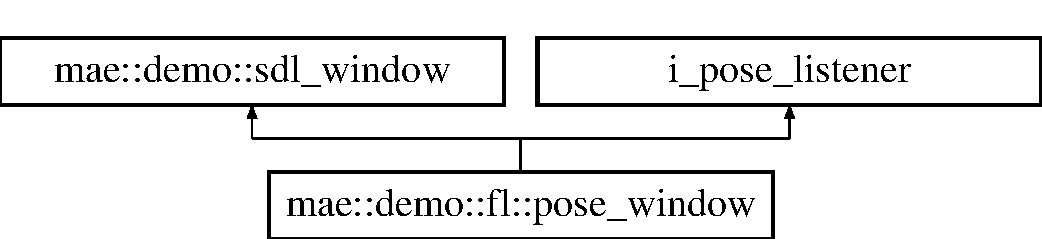
\includegraphics[height=2.000000cm]{classmae_1_1demo_1_1fl_1_1pose__window}
\end{center}
\end{figure}
\subsection*{Public Member Functions}
\begin{DoxyCompactItemize}
\item 
\hyperlink{classmae_1_1demo_1_1fl_1_1pose__window_a63d9c4c64ec9471438da845fa0d9b92b}{pose\-\_\-window} (std\-::string title, bool backgroundimage=false, int width=1024, int height=576, int x\-\_\-pos=S\-D\-L\-\_\-\-W\-I\-N\-D\-O\-W\-P\-O\-S\-\_\-\-U\-N\-D\-E\-F\-I\-N\-E\-D, int y\-\_\-pos=S\-D\-L\-\_\-\-W\-I\-N\-D\-O\-W\-P\-O\-S\-\_\-\-U\-N\-D\-E\-F\-I\-N\-E\-D, Uint32 flags=S\-D\-L\-\_\-\-W\-I\-N\-D\-O\-W\-\_\-\-S\-H\-O\-W\-N)
\item 
virtual void \hyperlink{classmae_1_1demo_1_1fl_1_1pose__window_adadc757a6ee3c70e3b3bf3500af6f60a}{on\-\_\-pose} (long timestamp, std\-::shared\-\_\-ptr$<$ general\-\_\-pose $>$ pose)
\end{DoxyCompactItemize}
\subsection*{Protected Member Functions}
\begin{DoxyCompactItemize}
\item 
virtual void \hyperlink{classmae_1_1demo_1_1fl_1_1pose__window_ab0677340d0c6b80216eb78467a02449d}{paint} (S\-D\-L\-\_\-\-Surface $\ast$graphics)
\item 
virtual void \hyperlink{classmae_1_1demo_1_1fl_1_1pose__window_af7734881adeb962b6119ae7548513541}{handle\-\_\-event} (S\-D\-L\-\_\-\-Event \&e)
\end{DoxyCompactItemize}
\subsection*{Additional Inherited Members}


\subsection{Constructor \& Destructor Documentation}
\hypertarget{classmae_1_1demo_1_1fl_1_1pose__window_a63d9c4c64ec9471438da845fa0d9b92b}{\index{mae\-::demo\-::fl\-::pose\-\_\-window@{mae\-::demo\-::fl\-::pose\-\_\-window}!pose\-\_\-window@{pose\-\_\-window}}
\index{pose\-\_\-window@{pose\-\_\-window}!mae::demo::fl::pose_window@{mae\-::demo\-::fl\-::pose\-\_\-window}}
\subsubsection[{pose\-\_\-window}]{\setlength{\rightskip}{0pt plus 5cm}mae\-::demo\-::fl\-::pose\-\_\-window\-::pose\-\_\-window (
\begin{DoxyParamCaption}
\item[{std\-::string}]{title, }
\item[{bool}]{backgroundimage = {\ttfamily false}, }
\item[{int}]{width = {\ttfamily 1024}, }
\item[{int}]{height = {\ttfamily 576}, }
\item[{int}]{x\-\_\-pos = {\ttfamily SDL\-\_\-WINDOWPOS\-\_\-UNDEFINED}, }
\item[{int}]{y\-\_\-pos = {\ttfamily SDL\-\_\-WINDOWPOS\-\_\-UNDEFINED}, }
\item[{Uint32}]{flags = {\ttfamily SDL\-\_\-WINDOW\-\_\-SHOWN}}
\end{DoxyParamCaption}
)}}\label{classmae_1_1demo_1_1fl_1_1pose__window_a63d9c4c64ec9471438da845fa0d9b92b}
Creates a window which shows poses for the input stream.


\begin{DoxyParams}{Parameters}
{\em title} & The window title. \\
\hline
{\em backgroundimage} & True if background image is desired. \\
\hline
{\em width} & The window's width. \\
\hline
{\em height} & The window's height. \\
\hline
{\em x\-\_\-pos} & The x position. \\
\hline
{\em y\-\_\-pos} & The y position. \\
\hline
{\em flags} & The window flags. \\
\hline
\end{DoxyParams}


\subsection{Member Function Documentation}
\hypertarget{classmae_1_1demo_1_1fl_1_1pose__window_af7734881adeb962b6119ae7548513541}{\index{mae\-::demo\-::fl\-::pose\-\_\-window@{mae\-::demo\-::fl\-::pose\-\_\-window}!handle\-\_\-event@{handle\-\_\-event}}
\index{handle\-\_\-event@{handle\-\_\-event}!mae::demo::fl::pose_window@{mae\-::demo\-::fl\-::pose\-\_\-window}}
\subsubsection[{handle\-\_\-event}]{\setlength{\rightskip}{0pt plus 5cm}void mae\-::demo\-::fl\-::pose\-\_\-window\-::handle\-\_\-event (
\begin{DoxyParamCaption}
\item[{S\-D\-L\-\_\-\-Event \&}]{e}
\end{DoxyParamCaption}
)\hspace{0.3cm}{\ttfamily [protected]}, {\ttfamily [virtual]}}}\label{classmae_1_1demo_1_1fl_1_1pose__window_af7734881adeb962b6119ae7548513541}
Paints content to the graphics element.


\begin{DoxyParams}{Parameters}
{\em graphics} & The graphics element. \\
\hline
\end{DoxyParams}


Reimplemented from \hyperlink{classmae_1_1demo_1_1sdl__window_a2bef43a55045075ff42c23a038245a5c}{mae\-::demo\-::sdl\-\_\-window}.

\hypertarget{classmae_1_1demo_1_1fl_1_1pose__window_adadc757a6ee3c70e3b3bf3500af6f60a}{\index{mae\-::demo\-::fl\-::pose\-\_\-window@{mae\-::demo\-::fl\-::pose\-\_\-window}!on\-\_\-pose@{on\-\_\-pose}}
\index{on\-\_\-pose@{on\-\_\-pose}!mae::demo::fl::pose_window@{mae\-::demo\-::fl\-::pose\-\_\-window}}
\subsubsection[{on\-\_\-pose}]{\setlength{\rightskip}{0pt plus 5cm}void mae\-::demo\-::fl\-::pose\-\_\-window\-::on\-\_\-pose (
\begin{DoxyParamCaption}
\item[{long}]{timestamp, }
\item[{std\-::shared\-\_\-ptr$<$ general\-\_\-pose $>$}]{pose}
\end{DoxyParamCaption}
)\hspace{0.3cm}{\ttfamily [virtual]}}}\label{classmae_1_1demo_1_1fl_1_1pose__window_adadc757a6ee3c70e3b3bf3500af6f60a}
Is invoked each time a pose was quantized (which occurs on every frame).


\begin{DoxyParams}{Parameters}
{\em timestamp} & The associated timestamp. \\
\hline
{\em pose} & The quantized pose. \\
\hline
\end{DoxyParams}
\hypertarget{classmae_1_1demo_1_1fl_1_1pose__window_ab0677340d0c6b80216eb78467a02449d}{\index{mae\-::demo\-::fl\-::pose\-\_\-window@{mae\-::demo\-::fl\-::pose\-\_\-window}!paint@{paint}}
\index{paint@{paint}!mae::demo::fl::pose_window@{mae\-::demo\-::fl\-::pose\-\_\-window}}
\subsubsection[{paint}]{\setlength{\rightskip}{0pt plus 5cm}void mae\-::demo\-::fl\-::pose\-\_\-window\-::paint (
\begin{DoxyParamCaption}
\item[{S\-D\-L\-\_\-\-Surface $\ast$}]{graphics}
\end{DoxyParamCaption}
)\hspace{0.3cm}{\ttfamily [protected]}, {\ttfamily [virtual]}}}\label{classmae_1_1demo_1_1fl_1_1pose__window_ab0677340d0c6b80216eb78467a02449d}
Handles the given event.


\begin{DoxyParams}{Parameters}
{\em e} & The event. \\
\hline
\end{DoxyParams}


Reimplemented from \hyperlink{classmae_1_1demo_1_1sdl__window_a3e9093b89993ebd52acbbc5d247750b8}{mae\-::demo\-::sdl\-\_\-window}.



The documentation for this class was generated from the following files\-:\begin{DoxyCompactItemize}
\item 
src/mae/demo/fl/pose\-\_\-window.\-hpp\item 
src/mae/demo/fl/pose\-\_\-window.\-cpp\end{DoxyCompactItemize}

\hypertarget{classmae_1_1demo_1_1fl_1_1recognition__window}{\section{mae\-:\-:demo\-:\-:fl\-:\-:recognition\-\_\-window Class Reference}
\label{classmae_1_1demo_1_1fl_1_1recognition__window}\index{mae\-::demo\-::fl\-::recognition\-\_\-window@{mae\-::demo\-::fl\-::recognition\-\_\-window}}
}
Inheritance diagram for mae\-:\-:demo\-:\-:fl\-:\-:recognition\-\_\-window\-:\begin{figure}[H]
\begin{center}
\leavevmode
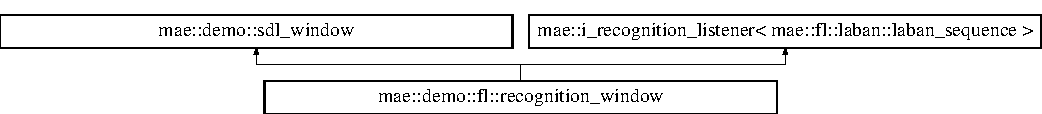
\includegraphics[height=1.534247cm]{classmae_1_1demo_1_1fl_1_1recognition__window}
\end{center}
\end{figure}
\subsection*{Public Member Functions}
\begin{DoxyCompactItemize}
\item 
\hyperlink{classmae_1_1demo_1_1fl_1_1recognition__window_a5eaeeccf36240c58df2aadeb6dd62439}{recognition\-\_\-window} (std\-::string title, bool backgroundimage=false, int width=1024, int height=576, int x\-\_\-pos=S\-D\-L\-\_\-\-W\-I\-N\-D\-O\-W\-P\-O\-S\-\_\-\-U\-N\-D\-E\-F\-I\-N\-E\-D, int y\-\_\-pos=S\-D\-L\-\_\-\-W\-I\-N\-D\-O\-W\-P\-O\-S\-\_\-\-U\-N\-D\-E\-F\-I\-N\-E\-D, Uint32 flags=S\-D\-L\-\_\-\-W\-I\-N\-D\-O\-W\-\_\-\-S\-H\-O\-W\-N)
\item 
virtual void \hyperlink{classmae_1_1demo_1_1fl_1_1recognition__window_a5f03f86740aac9b8c3f672d69d617bde}{on\-\_\-recognition} (long timestamp, std\-::vector$<$ std\-::shared\-\_\-ptr$<$ mae\-::fl\-::laban\-::laban\-\_\-sequence $>$ $>$ sequences)
\item 
virtual void \hyperlink{classmae_1_1demo_1_1fl_1_1recognition__window_a461cde34e9508178681124772dd1af08}{on\-\_\-recognition} (long timestamp, std\-::vector$<$ std\-::string $>$ title)
\end{DoxyCompactItemize}
\subsection*{Protected Member Functions}
\begin{DoxyCompactItemize}
\item 
virtual void \hyperlink{classmae_1_1demo_1_1fl_1_1recognition__window_a6be01c15215a8c705ebd5fe7b11f7b08}{paint} (S\-D\-L\-\_\-\-Surface $\ast$graphics)
\item 
virtual void \hyperlink{classmae_1_1demo_1_1fl_1_1recognition__window_a5ad1854bdbe05a3a7cc73c4a1b658236}{handle\-\_\-event} (S\-D\-L\-\_\-\-Event \&e)
\end{DoxyCompactItemize}
\subsection*{Additional Inherited Members}


\subsection{Constructor \& Destructor Documentation}
\hypertarget{classmae_1_1demo_1_1fl_1_1recognition__window_a5eaeeccf36240c58df2aadeb6dd62439}{\index{mae\-::demo\-::fl\-::recognition\-\_\-window@{mae\-::demo\-::fl\-::recognition\-\_\-window}!recognition\-\_\-window@{recognition\-\_\-window}}
\index{recognition\-\_\-window@{recognition\-\_\-window}!mae::demo::fl::recognition_window@{mae\-::demo\-::fl\-::recognition\-\_\-window}}
\subsubsection[{recognition\-\_\-window}]{\setlength{\rightskip}{0pt plus 5cm}mae\-::demo\-::fl\-::recognition\-\_\-window\-::recognition\-\_\-window (
\begin{DoxyParamCaption}
\item[{std\-::string}]{title, }
\item[{bool}]{backgroundimage = {\ttfamily false}, }
\item[{int}]{width = {\ttfamily 1024}, }
\item[{int}]{height = {\ttfamily 576}, }
\item[{int}]{x\-\_\-pos = {\ttfamily SDL\-\_\-WINDOWPOS\-\_\-UNDEFINED}, }
\item[{int}]{y\-\_\-pos = {\ttfamily SDL\-\_\-WINDOWPOS\-\_\-UNDEFINED}, }
\item[{Uint32}]{flags = {\ttfamily SDL\-\_\-WINDOW\-\_\-SHOWN}}
\end{DoxyParamCaption}
)}}\label{classmae_1_1demo_1_1fl_1_1recognition__window_a5eaeeccf36240c58df2aadeb6dd62439}
Creates a new S\-D\-L window for recognized laban\-\_\-sequences with the given parameters.

Must be invoked from the main thread.


\begin{DoxyParams}{Parameters}
{\em title} & The window title. \\
\hline
{\em backgroundimage} & True if background image is desired. \\
\hline
{\em width} & The window width. \\
\hline
{\em height} & The window height. \\
\hline
{\em x\-\_\-pos} & The window's x position. \\
\hline
{\em y\-\_\-pos} & The window's y position. \\
\hline
{\em flags} & The window flags. \\
\hline
\end{DoxyParams}


\subsection{Member Function Documentation}
\hypertarget{classmae_1_1demo_1_1fl_1_1recognition__window_a5ad1854bdbe05a3a7cc73c4a1b658236}{\index{mae\-::demo\-::fl\-::recognition\-\_\-window@{mae\-::demo\-::fl\-::recognition\-\_\-window}!handle\-\_\-event@{handle\-\_\-event}}
\index{handle\-\_\-event@{handle\-\_\-event}!mae::demo::fl::recognition_window@{mae\-::demo\-::fl\-::recognition\-\_\-window}}
\subsubsection[{handle\-\_\-event}]{\setlength{\rightskip}{0pt plus 5cm}void mae\-::demo\-::fl\-::recognition\-\_\-window\-::handle\-\_\-event (
\begin{DoxyParamCaption}
\item[{S\-D\-L\-\_\-\-Event \&}]{e}
\end{DoxyParamCaption}
)\hspace{0.3cm}{\ttfamily [protected]}, {\ttfamily [virtual]}}}\label{classmae_1_1demo_1_1fl_1_1recognition__window_a5ad1854bdbe05a3a7cc73c4a1b658236}
Paints content to the graphics element.


\begin{DoxyParams}{Parameters}
{\em graphics} & The graphics element. \\
\hline
\end{DoxyParams}


Reimplemented from \hyperlink{classmae_1_1demo_1_1sdl__window_a2bef43a55045075ff42c23a038245a5c}{mae\-::demo\-::sdl\-\_\-window}.

\hypertarget{classmae_1_1demo_1_1fl_1_1recognition__window_a5f03f86740aac9b8c3f672d69d617bde}{\index{mae\-::demo\-::fl\-::recognition\-\_\-window@{mae\-::demo\-::fl\-::recognition\-\_\-window}!on\-\_\-recognition@{on\-\_\-recognition}}
\index{on\-\_\-recognition@{on\-\_\-recognition}!mae::demo::fl::recognition_window@{mae\-::demo\-::fl\-::recognition\-\_\-window}}
\subsubsection[{on\-\_\-recognition}]{\setlength{\rightskip}{0pt plus 5cm}void mae\-::demo\-::fl\-::recognition\-\_\-window\-::on\-\_\-recognition (
\begin{DoxyParamCaption}
\item[{long}]{timestamp, }
\item[{std\-::vector$<$ std\-::shared\-\_\-ptr$<$ mae\-::fl\-::laban\-::laban\-\_\-sequence $>$ $>$}]{sequences}
\end{DoxyParamCaption}
)\hspace{0.3cm}{\ttfamily [virtual]}}}\label{classmae_1_1demo_1_1fl_1_1recognition__window_a5f03f86740aac9b8c3f672d69d617bde}
Is invoked each time sequences were recognized and the sequences are present.


\begin{DoxyParams}{Parameters}
{\em timestamp} & The associated timestamp. \\
\hline
{\em sequences} & The recognized sequences. \\
\hline
\end{DoxyParams}
\hypertarget{classmae_1_1demo_1_1fl_1_1recognition__window_a461cde34e9508178681124772dd1af08}{\index{mae\-::demo\-::fl\-::recognition\-\_\-window@{mae\-::demo\-::fl\-::recognition\-\_\-window}!on\-\_\-recognition@{on\-\_\-recognition}}
\index{on\-\_\-recognition@{on\-\_\-recognition}!mae::demo::fl::recognition_window@{mae\-::demo\-::fl\-::recognition\-\_\-window}}
\subsubsection[{on\-\_\-recognition}]{\setlength{\rightskip}{0pt plus 5cm}void mae\-::demo\-::fl\-::recognition\-\_\-window\-::on\-\_\-recognition (
\begin{DoxyParamCaption}
\item[{long}]{timestamp, }
\item[{std\-::vector$<$ std\-::string $>$}]{title}
\end{DoxyParamCaption}
)\hspace{0.3cm}{\ttfamily [virtual]}}}\label{classmae_1_1demo_1_1fl_1_1recognition__window_a461cde34e9508178681124772dd1af08}
Is invoked each time sequences were recognized and only titles of the sequences are present.


\begin{DoxyParams}{Parameters}
{\em timestamp} & The associated timestamp. \\
\hline
{\em sequences} & The recognized sequences. \\
\hline
\end{DoxyParams}
\hypertarget{classmae_1_1demo_1_1fl_1_1recognition__window_a6be01c15215a8c705ebd5fe7b11f7b08}{\index{mae\-::demo\-::fl\-::recognition\-\_\-window@{mae\-::demo\-::fl\-::recognition\-\_\-window}!paint@{paint}}
\index{paint@{paint}!mae::demo::fl::recognition_window@{mae\-::demo\-::fl\-::recognition\-\_\-window}}
\subsubsection[{paint}]{\setlength{\rightskip}{0pt plus 5cm}void mae\-::demo\-::fl\-::recognition\-\_\-window\-::paint (
\begin{DoxyParamCaption}
\item[{S\-D\-L\-\_\-\-Surface $\ast$}]{graphics}
\end{DoxyParamCaption}
)\hspace{0.3cm}{\ttfamily [protected]}, {\ttfamily [virtual]}}}\label{classmae_1_1demo_1_1fl_1_1recognition__window_a6be01c15215a8c705ebd5fe7b11f7b08}
Handles the given event.


\begin{DoxyParams}{Parameters}
{\em e} & The event. \\
\hline
\end{DoxyParams}


Reimplemented from \hyperlink{classmae_1_1demo_1_1sdl__window_a3e9093b89993ebd52acbbc5d247750b8}{mae\-::demo\-::sdl\-\_\-window}.



The documentation for this class was generated from the following files\-:\begin{DoxyCompactItemize}
\item 
src/mae/demo/fl/recognition\-\_\-window.\-hpp\item 
src/mae/demo/fl/recognition\-\_\-window.\-cpp\end{DoxyCompactItemize}

\hypertarget{classmae_1_1demo_1_1fl_1_1recorder__window}{\section{mae\-:\-:demo\-:\-:fl\-:\-:recorder\-\_\-window Class Reference}
\label{classmae_1_1demo_1_1fl_1_1recorder__window}\index{mae\-::demo\-::fl\-::recorder\-\_\-window@{mae\-::demo\-::fl\-::recorder\-\_\-window}}
}
Inheritance diagram for mae\-:\-:demo\-:\-:fl\-:\-:recorder\-\_\-window\-:\begin{figure}[H]
\begin{center}
\leavevmode
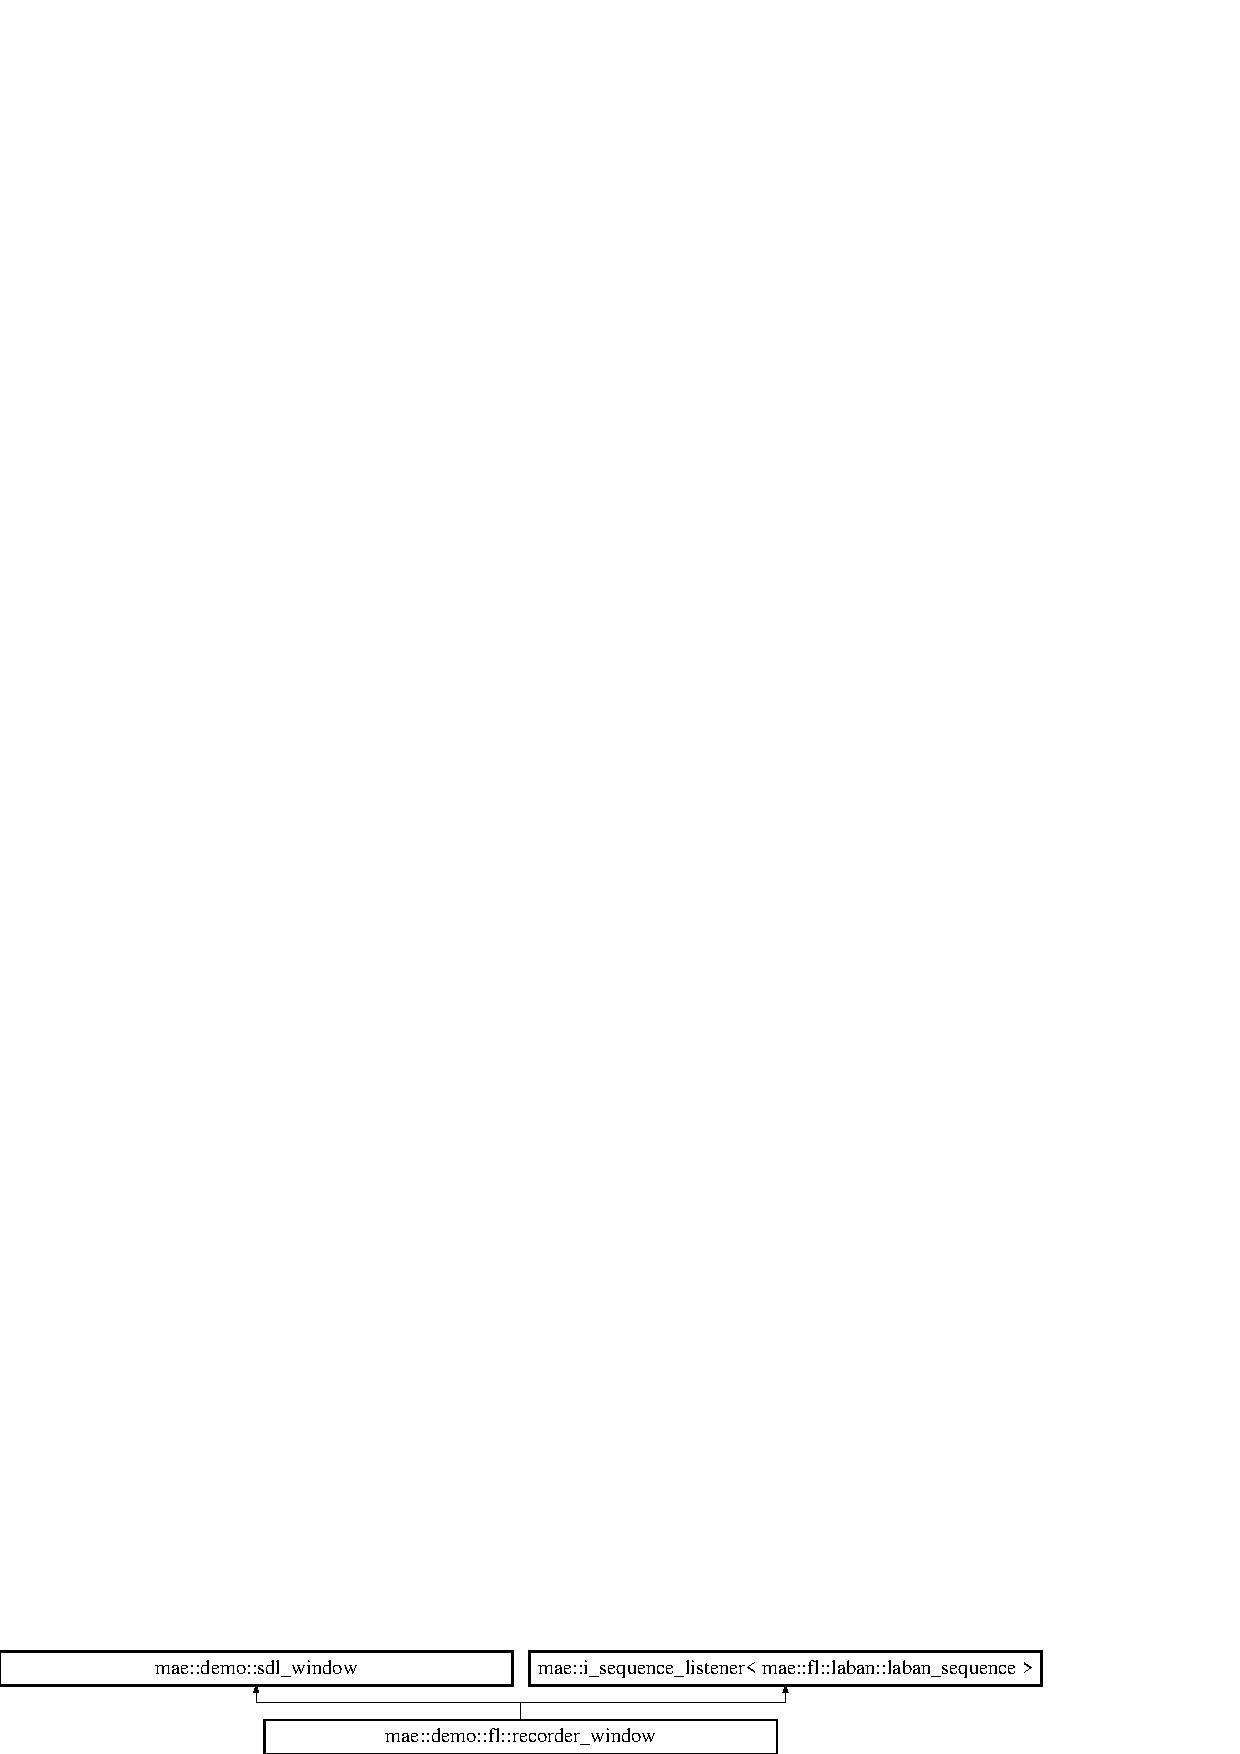
\includegraphics[height=1.573034cm]{classmae_1_1demo_1_1fl_1_1recorder__window}
\end{center}
\end{figure}
\subsection*{Public Member Functions}
\begin{DoxyCompactItemize}
\item 
\hyperlink{classmae_1_1demo_1_1fl_1_1recorder__window_a1dcfdfb8593efeac945b182a47c506c0}{recorder\-\_\-window} (std\-::string title, bool backgroundimage=false, int width=1024, int height=576, int x\-\_\-pos=S\-D\-L\-\_\-\-W\-I\-N\-D\-O\-W\-P\-O\-S\-\_\-\-U\-N\-D\-E\-F\-I\-N\-E\-D, int y\-\_\-pos=S\-D\-L\-\_\-\-W\-I\-N\-D\-O\-W\-P\-O\-S\-\_\-\-U\-N\-D\-E\-F\-I\-N\-E\-D, Uint32 flags=S\-D\-L\-\_\-\-W\-I\-N\-D\-O\-W\-\_\-\-S\-H\-O\-W\-N)
\item 
virtual void \hyperlink{classmae_1_1demo_1_1fl_1_1recorder__window_a2025de4acaea6121fe24baf340f4d7ce}{update\-\_\-countdown} (int time\-\_\-left)
\item 
virtual void \hyperlink{classmae_1_1demo_1_1fl_1_1recorder__window_a78ae661b3078f116b0b9cd80c0aac053}{clear\-\_\-paint} ()
\item 
virtual void \hyperlink{classmae_1_1demo_1_1fl_1_1recorder__window_a33b7253a227732d174513fecd312844b}{on\-\_\-sequence} (long timestamp, std\-::shared\-\_\-ptr$<$ mae\-::fl\-::laban\-::laban\-\_\-sequence $>$ sequence)
\end{DoxyCompactItemize}
\subsection*{Protected Member Functions}
\begin{DoxyCompactItemize}
\item 
virtual void \hyperlink{classmae_1_1demo_1_1fl_1_1recorder__window_a8f3e432809d394355c6a78398bba74c1}{paint} (S\-D\-L\-\_\-\-Surface $\ast$graphics)
\item 
virtual void \hyperlink{classmae_1_1demo_1_1fl_1_1recorder__window_ac937214271dbb036343530321e2762b7}{handle\-\_\-event} (S\-D\-L\-\_\-\-Event \&e)
\end{DoxyCompactItemize}
\subsection*{Additional Inherited Members}


\subsection{Constructor \& Destructor Documentation}
\hypertarget{classmae_1_1demo_1_1fl_1_1recorder__window_a1dcfdfb8593efeac945b182a47c506c0}{\index{mae\-::demo\-::fl\-::recorder\-\_\-window@{mae\-::demo\-::fl\-::recorder\-\_\-window}!recorder\-\_\-window@{recorder\-\_\-window}}
\index{recorder\-\_\-window@{recorder\-\_\-window}!mae::demo::fl::recorder_window@{mae\-::demo\-::fl\-::recorder\-\_\-window}}
\subsubsection[{recorder\-\_\-window}]{\setlength{\rightskip}{0pt plus 5cm}mae\-::demo\-::fl\-::recorder\-\_\-window\-::recorder\-\_\-window (
\begin{DoxyParamCaption}
\item[{std\-::string}]{title, }
\item[{bool}]{backgroundimage = {\ttfamily false}, }
\item[{int}]{width = {\ttfamily 1024}, }
\item[{int}]{height = {\ttfamily 576}, }
\item[{int}]{x\-\_\-pos = {\ttfamily SDL\-\_\-WINDOWPOS\-\_\-UNDEFINED}, }
\item[{int}]{y\-\_\-pos = {\ttfamily SDL\-\_\-WINDOWPOS\-\_\-UNDEFINED}, }
\item[{Uint32}]{flags = {\ttfamily SDL\-\_\-WINDOW\-\_\-SHOWN}}
\end{DoxyParamCaption}
)}}\label{classmae_1_1demo_1_1fl_1_1recorder__window_a1dcfdfb8593efeac945b182a47c506c0}
Creates a new recorder window to print countdowns and the currently recorded sequence.

Must be invoked from the main thread.


\begin{DoxyParams}{Parameters}
{\em title} & The window title. \\
\hline
{\em backgroundimage} & True if background image is desired. \\
\hline
{\em width} & The width. \\
\hline
{\em height} & The height. \\
\hline
{\em x\-\_\-pos} & The x pos. \\
\hline
{\em y\-\_\-pos} & The y pos. \\
\hline
{\em flags} & The flags to be applied. \\
\hline
\end{DoxyParams}


\subsection{Member Function Documentation}
\hypertarget{classmae_1_1demo_1_1fl_1_1recorder__window_a78ae661b3078f116b0b9cd80c0aac053}{\index{mae\-::demo\-::fl\-::recorder\-\_\-window@{mae\-::demo\-::fl\-::recorder\-\_\-window}!clear\-\_\-paint@{clear\-\_\-paint}}
\index{clear\-\_\-paint@{clear\-\_\-paint}!mae::demo::fl::recorder_window@{mae\-::demo\-::fl\-::recorder\-\_\-window}}
\subsubsection[{clear\-\_\-paint}]{\setlength{\rightskip}{0pt plus 5cm}void mae\-::demo\-::fl\-::recorder\-\_\-window\-::clear\-\_\-paint (
\begin{DoxyParamCaption}
{}
\end{DoxyParamCaption}
)\hspace{0.3cm}{\ttfamily [virtual]}}}\label{classmae_1_1demo_1_1fl_1_1recorder__window_a78ae661b3078f116b0b9cd80c0aac053}
Clears the graphics and removes the current sequence. \hypertarget{classmae_1_1demo_1_1fl_1_1recorder__window_ac937214271dbb036343530321e2762b7}{\index{mae\-::demo\-::fl\-::recorder\-\_\-window@{mae\-::demo\-::fl\-::recorder\-\_\-window}!handle\-\_\-event@{handle\-\_\-event}}
\index{handle\-\_\-event@{handle\-\_\-event}!mae::demo::fl::recorder_window@{mae\-::demo\-::fl\-::recorder\-\_\-window}}
\subsubsection[{handle\-\_\-event}]{\setlength{\rightskip}{0pt plus 5cm}void mae\-::demo\-::fl\-::recorder\-\_\-window\-::handle\-\_\-event (
\begin{DoxyParamCaption}
\item[{S\-D\-L\-\_\-\-Event \&}]{e}
\end{DoxyParamCaption}
)\hspace{0.3cm}{\ttfamily [protected]}, {\ttfamily [virtual]}}}\label{classmae_1_1demo_1_1fl_1_1recorder__window_ac937214271dbb036343530321e2762b7}
Paints content to the graphics element.


\begin{DoxyParams}{Parameters}
{\em graphics} & The graphics element. \\
\hline
\end{DoxyParams}


Reimplemented from \hyperlink{classmae_1_1demo_1_1sdl__window_a2bef43a55045075ff42c23a038245a5c}{mae\-::demo\-::sdl\-\_\-window}.

\hypertarget{classmae_1_1demo_1_1fl_1_1recorder__window_a33b7253a227732d174513fecd312844b}{\index{mae\-::demo\-::fl\-::recorder\-\_\-window@{mae\-::demo\-::fl\-::recorder\-\_\-window}!on\-\_\-sequence@{on\-\_\-sequence}}
\index{on\-\_\-sequence@{on\-\_\-sequence}!mae::demo::fl::recorder_window@{mae\-::demo\-::fl\-::recorder\-\_\-window}}
\subsubsection[{on\-\_\-sequence}]{\setlength{\rightskip}{0pt plus 5cm}void mae\-::demo\-::fl\-::recorder\-\_\-window\-::on\-\_\-sequence (
\begin{DoxyParamCaption}
\item[{long}]{timestamp, }
\item[{std\-::shared\-\_\-ptr$<$ mae\-::fl\-::laban\-::laban\-\_\-sequence $>$}]{sequence}
\end{DoxyParamCaption}
)\hspace{0.3cm}{\ttfamily [virtual]}}}\label{classmae_1_1demo_1_1fl_1_1recorder__window_a33b7253a227732d174513fecd312844b}
Is invoked each time a sequence was generated (which occurs on every frame).


\begin{DoxyParams}{Parameters}
{\em timestamp} & The associated timestamp. \\
\hline
{\em sequence} & The generated sequence. \\
\hline
\end{DoxyParams}
\hypertarget{classmae_1_1demo_1_1fl_1_1recorder__window_a8f3e432809d394355c6a78398bba74c1}{\index{mae\-::demo\-::fl\-::recorder\-\_\-window@{mae\-::demo\-::fl\-::recorder\-\_\-window}!paint@{paint}}
\index{paint@{paint}!mae::demo::fl::recorder_window@{mae\-::demo\-::fl\-::recorder\-\_\-window}}
\subsubsection[{paint}]{\setlength{\rightskip}{0pt plus 5cm}void mae\-::demo\-::fl\-::recorder\-\_\-window\-::paint (
\begin{DoxyParamCaption}
\item[{S\-D\-L\-\_\-\-Surface $\ast$}]{graphics}
\end{DoxyParamCaption}
)\hspace{0.3cm}{\ttfamily [protected]}, {\ttfamily [virtual]}}}\label{classmae_1_1demo_1_1fl_1_1recorder__window_a8f3e432809d394355c6a78398bba74c1}
Handles the given event.


\begin{DoxyParams}{Parameters}
{\em e} & The event. \\
\hline
\end{DoxyParams}


Reimplemented from \hyperlink{classmae_1_1demo_1_1sdl__window_a3e9093b89993ebd52acbbc5d247750b8}{mae\-::demo\-::sdl\-\_\-window}.

\hypertarget{classmae_1_1demo_1_1fl_1_1recorder__window_a2025de4acaea6121fe24baf340f4d7ce}{\index{mae\-::demo\-::fl\-::recorder\-\_\-window@{mae\-::demo\-::fl\-::recorder\-\_\-window}!update\-\_\-countdown@{update\-\_\-countdown}}
\index{update\-\_\-countdown@{update\-\_\-countdown}!mae::demo::fl::recorder_window@{mae\-::demo\-::fl\-::recorder\-\_\-window}}
\subsubsection[{update\-\_\-countdown}]{\setlength{\rightskip}{0pt plus 5cm}void mae\-::demo\-::fl\-::recorder\-\_\-window\-::update\-\_\-countdown (
\begin{DoxyParamCaption}
\item[{int}]{time\-\_\-left}
\end{DoxyParamCaption}
)\hspace{0.3cm}{\ttfamily [virtual]}}}\label{classmae_1_1demo_1_1fl_1_1recorder__window_a2025de4acaea6121fe24baf340f4d7ce}
Updates the countdown. If the countdown is -\/1 the drawing will be cleared. 
\begin{DoxyParams}{Parameters}
{\em time\-\_\-left} & \\
\hline
\end{DoxyParams}


The documentation for this class was generated from the following files\-:\begin{DoxyCompactItemize}
\item 
src/mae/demo/fl/recorder\-\_\-window.\-hpp\item 
src/mae/demo/fl/recorder\-\_\-window.\-cpp\end{DoxyCompactItemize}

\hypertarget{classmae_1_1demo_1_1sdl__window}{\section{mae\-:\-:demo\-:\-:sdl\-\_\-window Class Reference}
\label{classmae_1_1demo_1_1sdl__window}\index{mae\-::demo\-::sdl\-\_\-window@{mae\-::demo\-::sdl\-\_\-window}}
}
Inheritance diagram for mae\-:\-:demo\-:\-:sdl\-\_\-window\-:\begin{figure}[H]
\begin{center}
\leavevmode
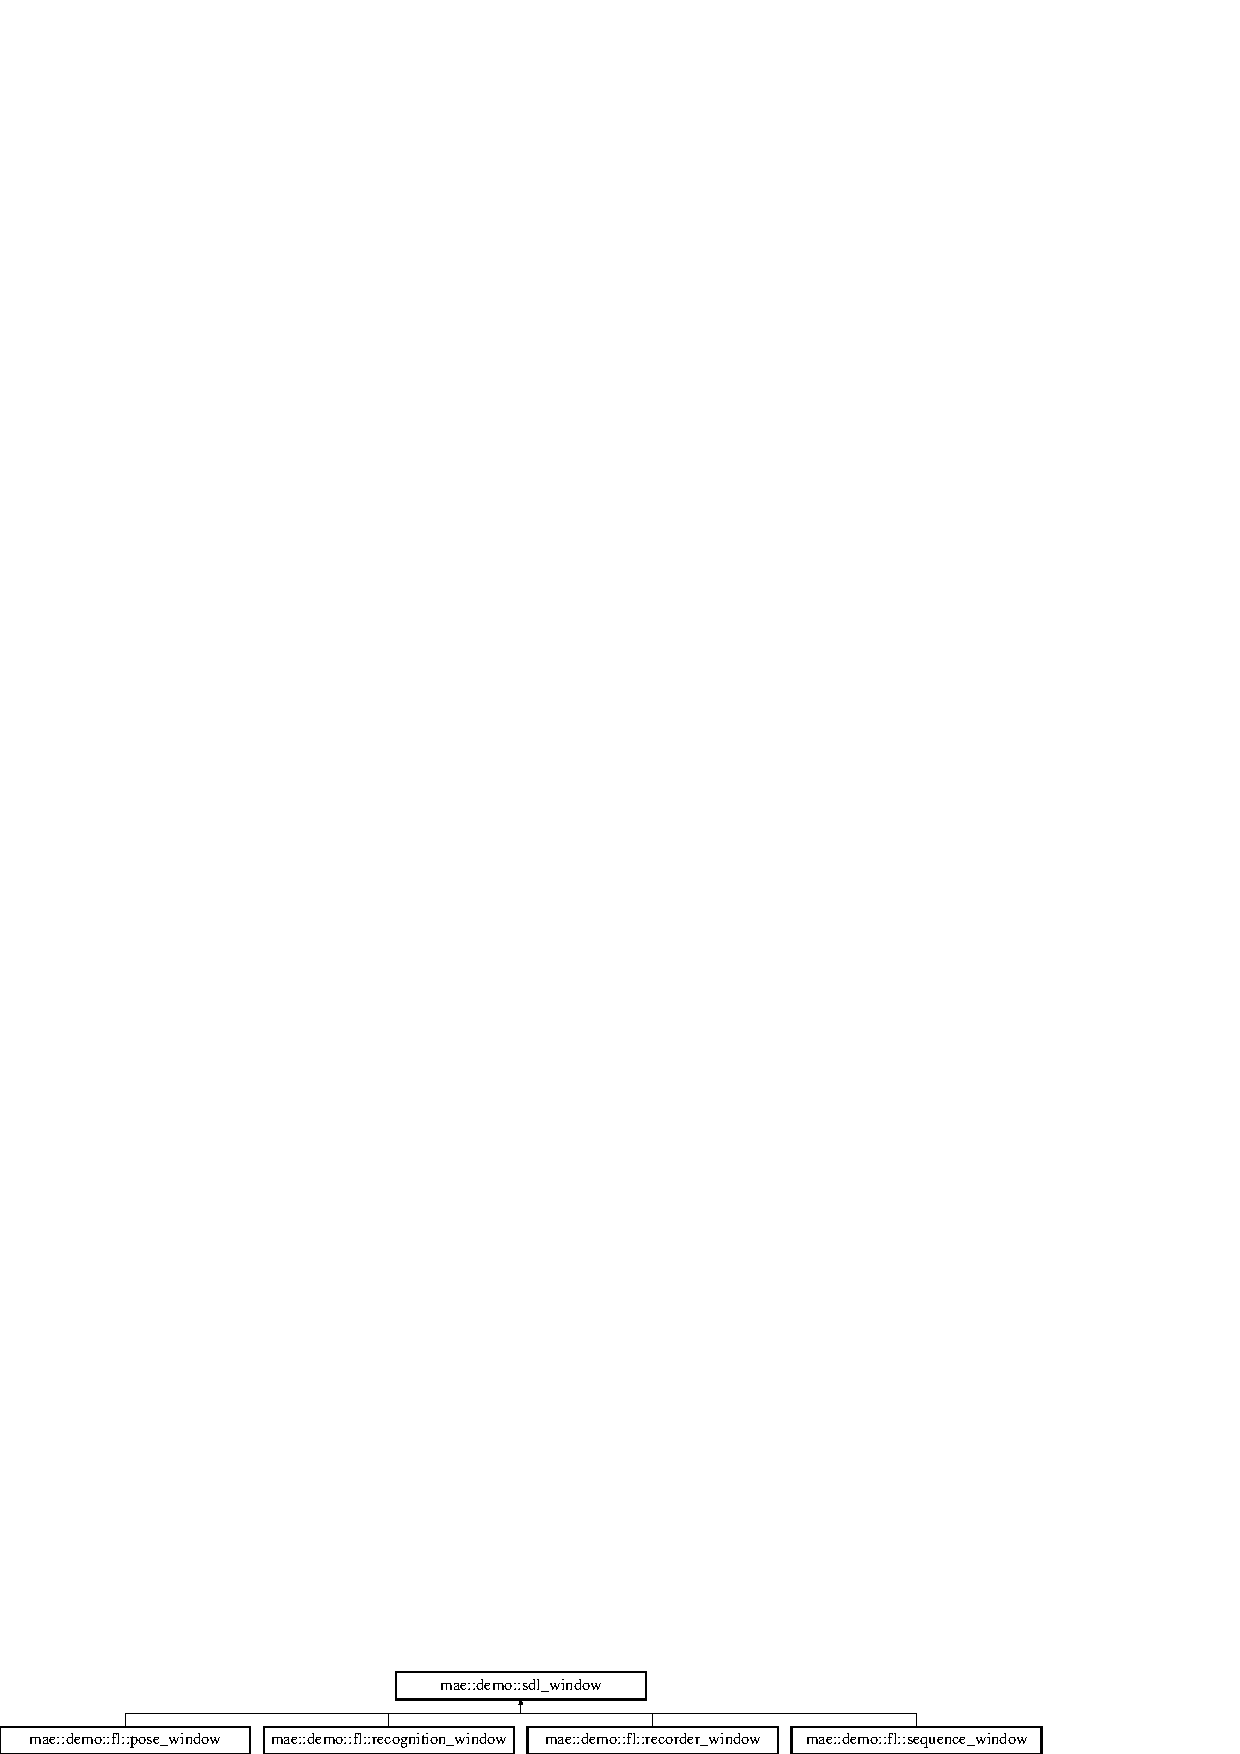
\includegraphics[height=1.333333cm]{classmae_1_1demo_1_1sdl__window}
\end{center}
\end{figure}
\subsection*{Public Member Functions}
\begin{DoxyCompactItemize}
\item 
\hyperlink{classmae_1_1demo_1_1sdl__window_a3c802b59d8f4461d747a165bd6786862}{sdl\-\_\-window} (std\-::string title, int width, int height, int x\-\_\-pos=S\-D\-L\-\_\-\-W\-I\-N\-D\-O\-W\-P\-O\-S\-\_\-\-U\-N\-D\-E\-F\-I\-N\-E\-D, int y\-\_\-pos=S\-D\-L\-\_\-\-W\-I\-N\-D\-O\-W\-P\-O\-S\-\_\-\-U\-N\-D\-E\-F\-I\-N\-E\-D, Uint32 flags=S\-D\-L\-\_\-\-W\-I\-N\-D\-O\-W\-\_\-\-S\-H\-O\-W\-N)
\item 
virtual void \hyperlink{classmae_1_1demo_1_1sdl__window_af4f9f15b3baa505c00a5fbb3f6c5c1db}{set\-\_\-title} (std\-::string title)
\item 
virtual std\-::string \hyperlink{classmae_1_1demo_1_1sdl__window_a4bb53fb50abd533e59342172b11631be}{get\-\_\-title} () const 
\item 
virtual void \hyperlink{classmae_1_1demo_1_1sdl__window_a1d2ca79353122cf7e9be5b834bfe1ec8}{set\-\_\-width} (int width)
\item 
virtual int \hyperlink{classmae_1_1demo_1_1sdl__window_ac14292ab54e1826e2d1ea17257ed607e}{get\-\_\-width} () const 
\item 
virtual void \hyperlink{classmae_1_1demo_1_1sdl__window_a6cfe2a0f1c777d7103a2c022d32ce615}{set\-\_\-height} (int height)
\item 
virtual int \hyperlink{classmae_1_1demo_1_1sdl__window_a0c0c633b3b292d7ce17ca88a466d2594}{get\-\_\-height} () const 
\item 
void \hyperlink{classmae_1_1demo_1_1sdl__window_a7e176a5cd6500918cb2a84d41a70a19b}{set\-\_\-size} (int width, int height)
\item 
virtual void \hyperlink{classmae_1_1demo_1_1sdl__window_a8543ba89320e1fa71f62f5d89a24d427}{repaint} ()
\item 
virtual bool \hyperlink{classmae_1_1demo_1_1sdl__window_aecc803312065a285c4f0b30f553a0e1d}{is\-\_\-repaint\-\_\-requested} () const 
\item 
virtual S\-D\-L\-\_\-\-Window $\ast$ \hyperlink{classmae_1_1demo_1_1sdl__window_afc849bc26aada2e22ee79b34ac686aec}{get} () const 
\item 
virtual S\-D\-L\-\_\-\-Surface $\ast$ \hyperlink{classmae_1_1demo_1_1sdl__window_a0ea2b4e2abd4d778b00f9e6281cff2c9}{get\-\_\-surface} () const 
\item 
virtual void \hyperlink{classmae_1_1demo_1_1sdl__window_a14893bb7b3868f605d8d39ff733929f0}{close} ()
\item 
virtual bool \hyperlink{classmae_1_1demo_1_1sdl__window_a4fcd254dfc2e0347d157200707c69fdb}{is\-\_\-closed} () const 
\end{DoxyCompactItemize}
\subsection*{Static Public Member Functions}
\begin{DoxyCompactItemize}
\item 
static void \hyperlink{classmae_1_1demo_1_1sdl__window_afd84acffe38cc8c0604c32b334198d1b}{update} ()
\end{DoxyCompactItemize}
\subsection*{Protected Member Functions}
\begin{DoxyCompactItemize}
\item 
virtual void \hyperlink{classmae_1_1demo_1_1sdl__window_a2bef43a55045075ff42c23a038245a5c}{handle\-\_\-event} (S\-D\-L\-\_\-\-Event \&e)
\item 
virtual void \hyperlink{classmae_1_1demo_1_1sdl__window_a3e9093b89993ebd52acbbc5d247750b8}{paint} (S\-D\-L\-\_\-\-Surface $\ast$graphics)
\item 
virtual void \hyperlink{classmae_1_1demo_1_1sdl__window_aac6f33798196668b0a0877c1466c013d}{do\-\_\-repaint} ()
\end{DoxyCompactItemize}


\subsection{Constructor \& Destructor Documentation}
\hypertarget{classmae_1_1demo_1_1sdl__window_a3c802b59d8f4461d747a165bd6786862}{\index{mae\-::demo\-::sdl\-\_\-window@{mae\-::demo\-::sdl\-\_\-window}!sdl\-\_\-window@{sdl\-\_\-window}}
\index{sdl\-\_\-window@{sdl\-\_\-window}!mae::demo::sdl_window@{mae\-::demo\-::sdl\-\_\-window}}
\subsubsection[{sdl\-\_\-window}]{\setlength{\rightskip}{0pt plus 5cm}mae\-::demo\-::sdl\-\_\-window\-::sdl\-\_\-window (
\begin{DoxyParamCaption}
\item[{std\-::string}]{title, }
\item[{int}]{width, }
\item[{int}]{height, }
\item[{int}]{x\-\_\-pos = {\ttfamily SDL\-\_\-WINDOWPOS\-\_\-UNDEFINED}, }
\item[{int}]{y\-\_\-pos = {\ttfamily SDL\-\_\-WINDOWPOS\-\_\-UNDEFINED}, }
\item[{Uint32}]{flags = {\ttfamily SDL\-\_\-WINDOW\-\_\-SHOWN}}
\end{DoxyParamCaption}
)}}\label{classmae_1_1demo_1_1sdl__window_a3c802b59d8f4461d747a165bd6786862}
Creates a new S\-D\-L window.

Must be invoked from the main thread.


\begin{DoxyParams}{Parameters}
{\em title} & The window title. \\
\hline
{\em width} & The window's width. \\
\hline
{\em height} & The window's height. \\
\hline
{\em x\-\_\-pos} & The window's x position. \\
\hline
{\em y\-\_\-pos} & The window's y position. \\
\hline
{\em flags} & The window flags. \\
\hline
\end{DoxyParams}


\subsection{Member Function Documentation}
\hypertarget{classmae_1_1demo_1_1sdl__window_a14893bb7b3868f605d8d39ff733929f0}{\index{mae\-::demo\-::sdl\-\_\-window@{mae\-::demo\-::sdl\-\_\-window}!close@{close}}
\index{close@{close}!mae::demo::sdl_window@{mae\-::demo\-::sdl\-\_\-window}}
\subsubsection[{close}]{\setlength{\rightskip}{0pt plus 5cm}void mae\-::demo\-::sdl\-\_\-window\-::close (
\begin{DoxyParamCaption}
{}
\end{DoxyParamCaption}
)\hspace{0.3cm}{\ttfamily [virtual]}}}\label{classmae_1_1demo_1_1sdl__window_a14893bb7b3868f605d8d39ff733929f0}
Closes the window. \hypertarget{classmae_1_1demo_1_1sdl__window_aac6f33798196668b0a0877c1466c013d}{\index{mae\-::demo\-::sdl\-\_\-window@{mae\-::demo\-::sdl\-\_\-window}!do\-\_\-repaint@{do\-\_\-repaint}}
\index{do\-\_\-repaint@{do\-\_\-repaint}!mae::demo::sdl_window@{mae\-::demo\-::sdl\-\_\-window}}
\subsubsection[{do\-\_\-repaint}]{\setlength{\rightskip}{0pt plus 5cm}void mae\-::demo\-::sdl\-\_\-window\-::do\-\_\-repaint (
\begin{DoxyParamCaption}
{}
\end{DoxyParamCaption}
)\hspace{0.3cm}{\ttfamily [protected]}, {\ttfamily [virtual]}}}\label{classmae_1_1demo_1_1sdl__window_aac6f33798196668b0a0877c1466c013d}
Does the actual repainting job. \hypertarget{classmae_1_1demo_1_1sdl__window_afc849bc26aada2e22ee79b34ac686aec}{\index{mae\-::demo\-::sdl\-\_\-window@{mae\-::demo\-::sdl\-\_\-window}!get@{get}}
\index{get@{get}!mae::demo::sdl_window@{mae\-::demo\-::sdl\-\_\-window}}
\subsubsection[{get}]{\setlength{\rightskip}{0pt plus 5cm}S\-D\-L\-\_\-\-Window $\ast$ mae\-::demo\-::sdl\-\_\-window\-::get (
\begin{DoxyParamCaption}
{}
\end{DoxyParamCaption}
) const\hspace{0.3cm}{\ttfamily [virtual]}}}\label{classmae_1_1demo_1_1sdl__window_afc849bc26aada2e22ee79b34ac686aec}
Returns the pointer to the S\-D\-L\-\_\-\-W\-I\-N\-D\-O\-W which remains valid until this object gets destroyed.

\begin{DoxyReturn}{Returns}
A pointer to the window. 
\end{DoxyReturn}
\hypertarget{classmae_1_1demo_1_1sdl__window_a0c0c633b3b292d7ce17ca88a466d2594}{\index{mae\-::demo\-::sdl\-\_\-window@{mae\-::demo\-::sdl\-\_\-window}!get\-\_\-height@{get\-\_\-height}}
\index{get\-\_\-height@{get\-\_\-height}!mae::demo::sdl_window@{mae\-::demo\-::sdl\-\_\-window}}
\subsubsection[{get\-\_\-height}]{\setlength{\rightskip}{0pt plus 5cm}int mae\-::demo\-::sdl\-\_\-window\-::get\-\_\-height (
\begin{DoxyParamCaption}
{}
\end{DoxyParamCaption}
) const\hspace{0.3cm}{\ttfamily [virtual]}}}\label{classmae_1_1demo_1_1sdl__window_a0c0c633b3b292d7ce17ca88a466d2594}
Returns the window's height.

\begin{DoxyReturn}{Returns}
The height. 
\end{DoxyReturn}
\hypertarget{classmae_1_1demo_1_1sdl__window_a0ea2b4e2abd4d778b00f9e6281cff2c9}{\index{mae\-::demo\-::sdl\-\_\-window@{mae\-::demo\-::sdl\-\_\-window}!get\-\_\-surface@{get\-\_\-surface}}
\index{get\-\_\-surface@{get\-\_\-surface}!mae::demo::sdl_window@{mae\-::demo\-::sdl\-\_\-window}}
\subsubsection[{get\-\_\-surface}]{\setlength{\rightskip}{0pt plus 5cm}S\-D\-L\-\_\-\-Surface $\ast$ mae\-::demo\-::sdl\-\_\-window\-::get\-\_\-surface (
\begin{DoxyParamCaption}
{}
\end{DoxyParamCaption}
) const\hspace{0.3cm}{\ttfamily [virtual]}}}\label{classmae_1_1demo_1_1sdl__window_a0ea2b4e2abd4d778b00f9e6281cff2c9}
Returns the pointer to the window's surface. \begin{DoxyReturn}{Returns}

\end{DoxyReturn}
\hypertarget{classmae_1_1demo_1_1sdl__window_a4bb53fb50abd533e59342172b11631be}{\index{mae\-::demo\-::sdl\-\_\-window@{mae\-::demo\-::sdl\-\_\-window}!get\-\_\-title@{get\-\_\-title}}
\index{get\-\_\-title@{get\-\_\-title}!mae::demo::sdl_window@{mae\-::demo\-::sdl\-\_\-window}}
\subsubsection[{get\-\_\-title}]{\setlength{\rightskip}{0pt plus 5cm}std\-::string mae\-::demo\-::sdl\-\_\-window\-::get\-\_\-title (
\begin{DoxyParamCaption}
{}
\end{DoxyParamCaption}
) const\hspace{0.3cm}{\ttfamily [virtual]}}}\label{classmae_1_1demo_1_1sdl__window_a4bb53fb50abd533e59342172b11631be}
Returns the window title.

\begin{DoxyReturn}{Returns}
The title. 
\end{DoxyReturn}
\hypertarget{classmae_1_1demo_1_1sdl__window_ac14292ab54e1826e2d1ea17257ed607e}{\index{mae\-::demo\-::sdl\-\_\-window@{mae\-::demo\-::sdl\-\_\-window}!get\-\_\-width@{get\-\_\-width}}
\index{get\-\_\-width@{get\-\_\-width}!mae::demo::sdl_window@{mae\-::demo\-::sdl\-\_\-window}}
\subsubsection[{get\-\_\-width}]{\setlength{\rightskip}{0pt plus 5cm}int mae\-::demo\-::sdl\-\_\-window\-::get\-\_\-width (
\begin{DoxyParamCaption}
{}
\end{DoxyParamCaption}
) const\hspace{0.3cm}{\ttfamily [virtual]}}}\label{classmae_1_1demo_1_1sdl__window_ac14292ab54e1826e2d1ea17257ed607e}
Returns the window's height.

\begin{DoxyReturn}{Returns}
The height. 
\end{DoxyReturn}
\hypertarget{classmae_1_1demo_1_1sdl__window_a2bef43a55045075ff42c23a038245a5c}{\index{mae\-::demo\-::sdl\-\_\-window@{mae\-::demo\-::sdl\-\_\-window}!handle\-\_\-event@{handle\-\_\-event}}
\index{handle\-\_\-event@{handle\-\_\-event}!mae::demo::sdl_window@{mae\-::demo\-::sdl\-\_\-window}}
\subsubsection[{handle\-\_\-event}]{\setlength{\rightskip}{0pt plus 5cm}void mae\-::demo\-::sdl\-\_\-window\-::handle\-\_\-event (
\begin{DoxyParamCaption}
\item[{S\-D\-L\-\_\-\-Event \&}]{e}
\end{DoxyParamCaption}
)\hspace{0.3cm}{\ttfamily [protected]}, {\ttfamily [virtual]}}}\label{classmae_1_1demo_1_1sdl__window_a2bef43a55045075ff42c23a038245a5c}
Handles the given event.


\begin{DoxyParams}{Parameters}
{\em e} & The event. \\
\hline
\end{DoxyParams}


Reimplemented in \hyperlink{classmae_1_1demo_1_1fl_1_1recognition__window_a5ad1854bdbe05a3a7cc73c4a1b658236}{mae\-::demo\-::fl\-::recognition\-\_\-window}, \hyperlink{classmae_1_1demo_1_1fl_1_1recorder__window_ac937214271dbb036343530321e2762b7}{mae\-::demo\-::fl\-::recorder\-\_\-window}, \hyperlink{classmae_1_1demo_1_1fl_1_1sequence__window_aa84337da46e012c45d49462641d61f55}{mae\-::demo\-::fl\-::sequence\-\_\-window}, and \hyperlink{classmae_1_1demo_1_1fl_1_1pose__window_af7734881adeb962b6119ae7548513541}{mae\-::demo\-::fl\-::pose\-\_\-window}.

\hypertarget{classmae_1_1demo_1_1sdl__window_a4fcd254dfc2e0347d157200707c69fdb}{\index{mae\-::demo\-::sdl\-\_\-window@{mae\-::demo\-::sdl\-\_\-window}!is\-\_\-closed@{is\-\_\-closed}}
\index{is\-\_\-closed@{is\-\_\-closed}!mae::demo::sdl_window@{mae\-::demo\-::sdl\-\_\-window}}
\subsubsection[{is\-\_\-closed}]{\setlength{\rightskip}{0pt plus 5cm}bool mae\-::demo\-::sdl\-\_\-window\-::is\-\_\-closed (
\begin{DoxyParamCaption}
{}
\end{DoxyParamCaption}
) const\hspace{0.3cm}{\ttfamily [virtual]}}}\label{classmae_1_1demo_1_1sdl__window_a4fcd254dfc2e0347d157200707c69fdb}
Returns true if the window is closed.

\begin{DoxyReturn}{Returns}
True if closed 
\end{DoxyReturn}
\hypertarget{classmae_1_1demo_1_1sdl__window_aecc803312065a285c4f0b30f553a0e1d}{\index{mae\-::demo\-::sdl\-\_\-window@{mae\-::demo\-::sdl\-\_\-window}!is\-\_\-repaint\-\_\-requested@{is\-\_\-repaint\-\_\-requested}}
\index{is\-\_\-repaint\-\_\-requested@{is\-\_\-repaint\-\_\-requested}!mae::demo::sdl_window@{mae\-::demo\-::sdl\-\_\-window}}
\subsubsection[{is\-\_\-repaint\-\_\-requested}]{\setlength{\rightskip}{0pt plus 5cm}bool mae\-::demo\-::sdl\-\_\-window\-::is\-\_\-repaint\-\_\-requested (
\begin{DoxyParamCaption}
{}
\end{DoxyParamCaption}
) const\hspace{0.3cm}{\ttfamily [virtual]}}}\label{classmae_1_1demo_1_1sdl__window_aecc803312065a285c4f0b30f553a0e1d}
Returns true if a repaint was requested recently.

\begin{DoxyReturn}{Returns}
True if repaint was requested. 
\end{DoxyReturn}
\hypertarget{classmae_1_1demo_1_1sdl__window_a3e9093b89993ebd52acbbc5d247750b8}{\index{mae\-::demo\-::sdl\-\_\-window@{mae\-::demo\-::sdl\-\_\-window}!paint@{paint}}
\index{paint@{paint}!mae::demo::sdl_window@{mae\-::demo\-::sdl\-\_\-window}}
\subsubsection[{paint}]{\setlength{\rightskip}{0pt plus 5cm}void mae\-::demo\-::sdl\-\_\-window\-::paint (
\begin{DoxyParamCaption}
\item[{S\-D\-L\-\_\-\-Surface $\ast$}]{graphics}
\end{DoxyParamCaption}
)\hspace{0.3cm}{\ttfamily [protected]}, {\ttfamily [virtual]}}}\label{classmae_1_1demo_1_1sdl__window_a3e9093b89993ebd52acbbc5d247750b8}
Paints content to the graphics element.


\begin{DoxyParams}{Parameters}
{\em graphics} & The graphics element. \\
\hline
\end{DoxyParams}


Reimplemented in \hyperlink{classmae_1_1demo_1_1fl_1_1recognition__window_a6be01c15215a8c705ebd5fe7b11f7b08}{mae\-::demo\-::fl\-::recognition\-\_\-window}, \hyperlink{classmae_1_1demo_1_1fl_1_1recorder__window_a8f3e432809d394355c6a78398bba74c1}{mae\-::demo\-::fl\-::recorder\-\_\-window}, \hyperlink{classmae_1_1demo_1_1fl_1_1sequence__window_ab70f1dfc88bf7c113f2b72f29bf9811d}{mae\-::demo\-::fl\-::sequence\-\_\-window}, and \hyperlink{classmae_1_1demo_1_1fl_1_1pose__window_ab0677340d0c6b80216eb78467a02449d}{mae\-::demo\-::fl\-::pose\-\_\-window}.

\hypertarget{classmae_1_1demo_1_1sdl__window_a8543ba89320e1fa71f62f5d89a24d427}{\index{mae\-::demo\-::sdl\-\_\-window@{mae\-::demo\-::sdl\-\_\-window}!repaint@{repaint}}
\index{repaint@{repaint}!mae::demo::sdl_window@{mae\-::demo\-::sdl\-\_\-window}}
\subsubsection[{repaint}]{\setlength{\rightskip}{0pt plus 5cm}void mae\-::demo\-::sdl\-\_\-window\-::repaint (
\begin{DoxyParamCaption}
{}
\end{DoxyParamCaption}
)\hspace{0.3cm}{\ttfamily [virtual]}}}\label{classmae_1_1demo_1_1sdl__window_a8543ba89320e1fa71f62f5d89a24d427}
Repaints the window's content. Invokes the paint method. \hypertarget{classmae_1_1demo_1_1sdl__window_a6cfe2a0f1c777d7103a2c022d32ce615}{\index{mae\-::demo\-::sdl\-\_\-window@{mae\-::demo\-::sdl\-\_\-window}!set\-\_\-height@{set\-\_\-height}}
\index{set\-\_\-height@{set\-\_\-height}!mae::demo::sdl_window@{mae\-::demo\-::sdl\-\_\-window}}
\subsubsection[{set\-\_\-height}]{\setlength{\rightskip}{0pt plus 5cm}void mae\-::demo\-::sdl\-\_\-window\-::set\-\_\-height (
\begin{DoxyParamCaption}
\item[{int}]{height}
\end{DoxyParamCaption}
)\hspace{0.3cm}{\ttfamily [virtual]}}}\label{classmae_1_1demo_1_1sdl__window_a6cfe2a0f1c777d7103a2c022d32ce615}
Sets the window's height.


\begin{DoxyParams}{Parameters}
{\em height} & The height. \\
\hline
\end{DoxyParams}
\hypertarget{classmae_1_1demo_1_1sdl__window_a7e176a5cd6500918cb2a84d41a70a19b}{\index{mae\-::demo\-::sdl\-\_\-window@{mae\-::demo\-::sdl\-\_\-window}!set\-\_\-size@{set\-\_\-size}}
\index{set\-\_\-size@{set\-\_\-size}!mae::demo::sdl_window@{mae\-::demo\-::sdl\-\_\-window}}
\subsubsection[{set\-\_\-size}]{\setlength{\rightskip}{0pt plus 5cm}void mae\-::demo\-::sdl\-\_\-window\-::set\-\_\-size (
\begin{DoxyParamCaption}
\item[{int}]{width, }
\item[{int}]{height}
\end{DoxyParamCaption}
)}}\label{classmae_1_1demo_1_1sdl__window_a7e176a5cd6500918cb2a84d41a70a19b}
Sets the window size.


\begin{DoxyParams}{Parameters}
{\em width} & The width to be applied. \\
\hline
{\em height} & The height to be applied. \\
\hline
\end{DoxyParams}
\hypertarget{classmae_1_1demo_1_1sdl__window_af4f9f15b3baa505c00a5fbb3f6c5c1db}{\index{mae\-::demo\-::sdl\-\_\-window@{mae\-::demo\-::sdl\-\_\-window}!set\-\_\-title@{set\-\_\-title}}
\index{set\-\_\-title@{set\-\_\-title}!mae::demo::sdl_window@{mae\-::demo\-::sdl\-\_\-window}}
\subsubsection[{set\-\_\-title}]{\setlength{\rightskip}{0pt plus 5cm}void mae\-::demo\-::sdl\-\_\-window\-::set\-\_\-title (
\begin{DoxyParamCaption}
\item[{std\-::string}]{title}
\end{DoxyParamCaption}
)\hspace{0.3cm}{\ttfamily [virtual]}}}\label{classmae_1_1demo_1_1sdl__window_af4f9f15b3baa505c00a5fbb3f6c5c1db}
Sets the window title.


\begin{DoxyParams}{Parameters}
{\em title} & The title. \\
\hline
\end{DoxyParams}
\hypertarget{classmae_1_1demo_1_1sdl__window_a1d2ca79353122cf7e9be5b834bfe1ec8}{\index{mae\-::demo\-::sdl\-\_\-window@{mae\-::demo\-::sdl\-\_\-window}!set\-\_\-width@{set\-\_\-width}}
\index{set\-\_\-width@{set\-\_\-width}!mae::demo::sdl_window@{mae\-::demo\-::sdl\-\_\-window}}
\subsubsection[{set\-\_\-width}]{\setlength{\rightskip}{0pt plus 5cm}void mae\-::demo\-::sdl\-\_\-window\-::set\-\_\-width (
\begin{DoxyParamCaption}
\item[{int}]{width}
\end{DoxyParamCaption}
)\hspace{0.3cm}{\ttfamily [virtual]}}}\label{classmae_1_1demo_1_1sdl__window_a1d2ca79353122cf7e9be5b834bfe1ec8}
Returns the window's width.


\begin{DoxyParams}{Parameters}
{\em width} & The width. \\
\hline
\end{DoxyParams}
\hypertarget{classmae_1_1demo_1_1sdl__window_afd84acffe38cc8c0604c32b334198d1b}{\index{mae\-::demo\-::sdl\-\_\-window@{mae\-::demo\-::sdl\-\_\-window}!update@{update}}
\index{update@{update}!mae::demo::sdl_window@{mae\-::demo\-::sdl\-\_\-window}}
\subsubsection[{update}]{\setlength{\rightskip}{0pt plus 5cm}void mae\-::demo\-::sdl\-\_\-window\-::update (
\begin{DoxyParamCaption}
{}
\end{DoxyParamCaption}
)\hspace{0.3cm}{\ttfamily [static]}}}\label{classmae_1_1demo_1_1sdl__window_afd84acffe38cc8c0604c32b334198d1b}
Updates all living windows. This includes polling events as well as repaint jobs.

This method must be invoked from the main thread of the program. 

The documentation for this class was generated from the following files\-:\begin{DoxyCompactItemize}
\item 
src/mae/demo/sdl\-\_\-window.\-hpp\item 
src/mae/demo/sdl\-\_\-window.\-cpp\end{DoxyCompactItemize}

\hypertarget{classmae_1_1demo_1_1sdl__window__item}{\section{mae\-:\-:demo\-:\-:sdl\-\_\-window\-\_\-item Class Reference}
\label{classmae_1_1demo_1_1sdl__window__item}\index{mae\-::demo\-::sdl\-\_\-window\-\_\-item@{mae\-::demo\-::sdl\-\_\-window\-\_\-item}}
}
\subsection*{Public Member Functions}
\begin{DoxyCompactItemize}
\item 
\hypertarget{classmae_1_1demo_1_1sdl__window__item_ad36eb63c7482082eaaf711ae02585bc2}{{\bfseries sdl\-\_\-window\-\_\-item} (std\-::string title, int width, int height, int x\-\_\-pos, int y\-\_\-pos, Uint32 flags)}\label{classmae_1_1demo_1_1sdl__window__item_ad36eb63c7482082eaaf711ae02585bc2}

\item 
\hypertarget{classmae_1_1demo_1_1sdl__window__item_a1c004e8cf8747b832e02cc51f0a72b98}{virtual std\-::string {\bfseries get\-\_\-title} ()}\label{classmae_1_1demo_1_1sdl__window__item_a1c004e8cf8747b832e02cc51f0a72b98}

\item 
\hypertarget{classmae_1_1demo_1_1sdl__window__item_a240121531269eb85c3a16eb0211fb5c6}{virtual int {\bfseries get\-\_\-width} ()}\label{classmae_1_1demo_1_1sdl__window__item_a240121531269eb85c3a16eb0211fb5c6}

\item 
\hypertarget{classmae_1_1demo_1_1sdl__window__item_adef11435c4b2ff565a93b8d604066e43}{virtual int {\bfseries get\-\_\-height} ()}\label{classmae_1_1demo_1_1sdl__window__item_adef11435c4b2ff565a93b8d604066e43}

\item 
\hypertarget{classmae_1_1demo_1_1sdl__window__item_ad29e8e44e7de4bb99b77990bc318227d}{virtual int {\bfseries get\-\_\-x\-\_\-pos} ()}\label{classmae_1_1demo_1_1sdl__window__item_ad29e8e44e7de4bb99b77990bc318227d}

\item 
\hypertarget{classmae_1_1demo_1_1sdl__window__item_aee9c4c7f51d96259cea2192feca979dc}{virtual int {\bfseries get\-\_\-y\-\_\-pos} ()}\label{classmae_1_1demo_1_1sdl__window__item_aee9c4c7f51d96259cea2192feca979dc}

\item 
\hypertarget{classmae_1_1demo_1_1sdl__window__item_a68e4d6296dd2e74a391a8ff27497a9c2}{virtual Uint32 {\bfseries get\-\_\-flags} ()}\label{classmae_1_1demo_1_1sdl__window__item_a68e4d6296dd2e74a391a8ff27497a9c2}

\item 
\hypertarget{classmae_1_1demo_1_1sdl__window__item_a60e090b82e1f7f75911da0ad20f62c1c}{virtual bool {\bfseries created} ()}\label{classmae_1_1demo_1_1sdl__window__item_a60e090b82e1f7f75911da0ad20f62c1c}

\item 
\hypertarget{classmae_1_1demo_1_1sdl__window__item_a8fe69e6a06e2c07db0f374a0b3b5dfae}{virtual bool {\bfseries exception} ()}\label{classmae_1_1demo_1_1sdl__window__item_a8fe69e6a06e2c07db0f374a0b3b5dfae}

\item 
\hypertarget{classmae_1_1demo_1_1sdl__window__item_a788db959668b4b3e1cfb454ea0be9ded}{virtual void {\bfseries set\-\_\-exception} (bool exception)}\label{classmae_1_1demo_1_1sdl__window__item_a788db959668b4b3e1cfb454ea0be9ded}

\item 
\hypertarget{classmae_1_1demo_1_1sdl__window__item_a77edff64e79daab7a717d789a8d848cf}{virtual void {\bfseries set\-\_\-created} (bool created)}\label{classmae_1_1demo_1_1sdl__window__item_a77edff64e79daab7a717d789a8d848cf}

\end{DoxyCompactItemize}


The documentation for this class was generated from the following files\-:\begin{DoxyCompactItemize}
\item 
src/mae/demo/sdl\-\_\-window\-\_\-item.\-hpp\item 
src/mae/demo/sdl\-\_\-window\-\_\-item.\-cpp\end{DoxyCompactItemize}

\hypertarget{classmae_1_1demo_1_1fl_1_1sequence__window}{\section{mae\-:\-:demo\-:\-:fl\-:\-:sequence\-\_\-window Class Reference}
\label{classmae_1_1demo_1_1fl_1_1sequence__window}\index{mae\-::demo\-::fl\-::sequence\-\_\-window@{mae\-::demo\-::fl\-::sequence\-\_\-window}}
}
Inheritance diagram for mae\-:\-:demo\-:\-:fl\-:\-:sequence\-\_\-window\-:\begin{figure}[H]
\begin{center}
\leavevmode
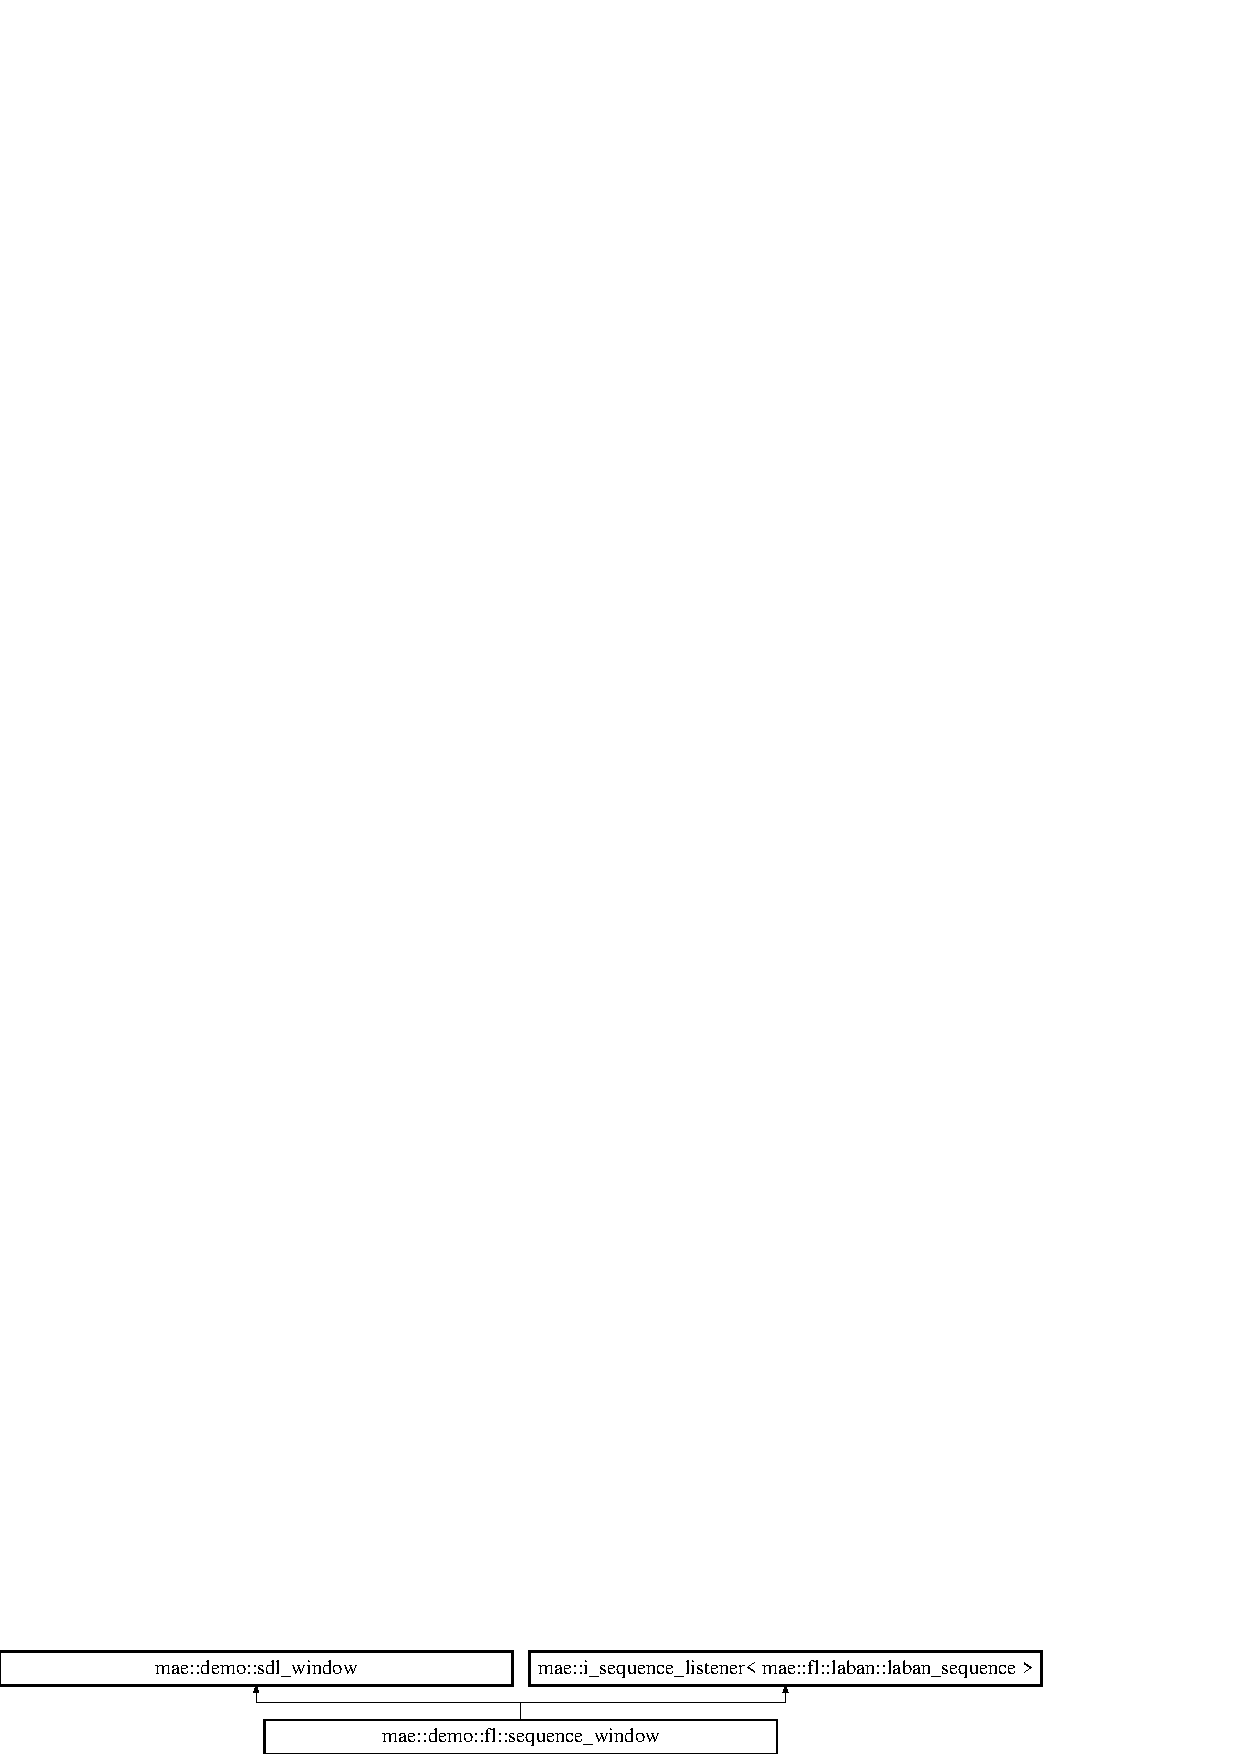
\includegraphics[height=1.573034cm]{classmae_1_1demo_1_1fl_1_1sequence__window}
\end{center}
\end{figure}
\subsection*{Public Member Functions}
\begin{DoxyCompactItemize}
\item 
\hyperlink{classmae_1_1demo_1_1fl_1_1sequence__window_a0f686b60ca61a3a328cd69e01912db09}{sequence\-\_\-window} (std\-::string title, bool backgroundimage=false, int width=1024, int height=576, int x\-\_\-pos=S\-D\-L\-\_\-\-W\-I\-N\-D\-O\-W\-P\-O\-S\-\_\-\-U\-N\-D\-E\-F\-I\-N\-E\-D, int y\-\_\-pos=S\-D\-L\-\_\-\-W\-I\-N\-D\-O\-W\-P\-O\-S\-\_\-\-U\-N\-D\-E\-F\-I\-N\-E\-D, Uint32 flags=S\-D\-L\-\_\-\-W\-I\-N\-D\-O\-W\-\_\-\-S\-H\-O\-W\-N)
\item 
virtual void \hyperlink{classmae_1_1demo_1_1fl_1_1sequence__window_a392112be053c0f58e9d26cb5b1d4109a}{on\-\_\-sequence} (long timestamp, std\-::shared\-\_\-ptr$<$ mae\-::fl\-::laban\-::laban\-\_\-sequence $>$ sequence)
\end{DoxyCompactItemize}
\subsection*{Protected Member Functions}
\begin{DoxyCompactItemize}
\item 
virtual void \hyperlink{classmae_1_1demo_1_1fl_1_1sequence__window_ab70f1dfc88bf7c113f2b72f29bf9811d}{paint} (S\-D\-L\-\_\-\-Surface $\ast$graphics)
\item 
virtual void \hyperlink{classmae_1_1demo_1_1fl_1_1sequence__window_aa84337da46e012c45d49462641d61f55}{handle\-\_\-event} (S\-D\-L\-\_\-\-Event \&e)
\end{DoxyCompactItemize}
\subsection*{Additional Inherited Members}


\subsection{Constructor \& Destructor Documentation}
\hypertarget{classmae_1_1demo_1_1fl_1_1sequence__window_a0f686b60ca61a3a328cd69e01912db09}{\index{mae\-::demo\-::fl\-::sequence\-\_\-window@{mae\-::demo\-::fl\-::sequence\-\_\-window}!sequence\-\_\-window@{sequence\-\_\-window}}
\index{sequence\-\_\-window@{sequence\-\_\-window}!mae::demo::fl::sequence_window@{mae\-::demo\-::fl\-::sequence\-\_\-window}}
\subsubsection[{sequence\-\_\-window}]{\setlength{\rightskip}{0pt plus 5cm}mae\-::demo\-::fl\-::sequence\-\_\-window\-::sequence\-\_\-window (
\begin{DoxyParamCaption}
\item[{std\-::string}]{title, }
\item[{bool}]{backgroundimage = {\ttfamily false}, }
\item[{int}]{width = {\ttfamily 1024}, }
\item[{int}]{height = {\ttfamily 576}, }
\item[{int}]{x\-\_\-pos = {\ttfamily SDL\-\_\-WINDOWPOS\-\_\-UNDEFINED}, }
\item[{int}]{y\-\_\-pos = {\ttfamily SDL\-\_\-WINDOWPOS\-\_\-UNDEFINED}, }
\item[{Uint32}]{flags = {\ttfamily SDL\-\_\-WINDOW\-\_\-SHOWN}}
\end{DoxyParamCaption}
)}}\label{classmae_1_1demo_1_1fl_1_1sequence__window_a0f686b60ca61a3a328cd69e01912db09}
Creates a new S\-D\-L window for generated laban\-\_\-sequences with the given parameters.

Must be invoked from the main thread.


\begin{DoxyParams}{Parameters}
{\em title} & The window title. \\
\hline
{\em backgroundimage} & True if background image is desired. \\
\hline
{\em width} & The window width. \\
\hline
{\em height} & The window height. \\
\hline
{\em x\-\_\-pos} & The window's x position. \\
\hline
{\em y\-\_\-pos} & The window's y position. \\
\hline
{\em flags} & The window flags. \\
\hline
\end{DoxyParams}


\subsection{Member Function Documentation}
\hypertarget{classmae_1_1demo_1_1fl_1_1sequence__window_aa84337da46e012c45d49462641d61f55}{\index{mae\-::demo\-::fl\-::sequence\-\_\-window@{mae\-::demo\-::fl\-::sequence\-\_\-window}!handle\-\_\-event@{handle\-\_\-event}}
\index{handle\-\_\-event@{handle\-\_\-event}!mae::demo::fl::sequence_window@{mae\-::demo\-::fl\-::sequence\-\_\-window}}
\subsubsection[{handle\-\_\-event}]{\setlength{\rightskip}{0pt plus 5cm}void mae\-::demo\-::fl\-::sequence\-\_\-window\-::handle\-\_\-event (
\begin{DoxyParamCaption}
\item[{S\-D\-L\-\_\-\-Event \&}]{e}
\end{DoxyParamCaption}
)\hspace{0.3cm}{\ttfamily [protected]}, {\ttfamily [virtual]}}}\label{classmae_1_1demo_1_1fl_1_1sequence__window_aa84337da46e012c45d49462641d61f55}
Paints content to the graphics element.


\begin{DoxyParams}{Parameters}
{\em graphics} & The graphics element. \\
\hline
\end{DoxyParams}


Reimplemented from \hyperlink{classmae_1_1demo_1_1sdl__window_a2bef43a55045075ff42c23a038245a5c}{mae\-::demo\-::sdl\-\_\-window}.

\hypertarget{classmae_1_1demo_1_1fl_1_1sequence__window_a392112be053c0f58e9d26cb5b1d4109a}{\index{mae\-::demo\-::fl\-::sequence\-\_\-window@{mae\-::demo\-::fl\-::sequence\-\_\-window}!on\-\_\-sequence@{on\-\_\-sequence}}
\index{on\-\_\-sequence@{on\-\_\-sequence}!mae::demo::fl::sequence_window@{mae\-::demo\-::fl\-::sequence\-\_\-window}}
\subsubsection[{on\-\_\-sequence}]{\setlength{\rightskip}{0pt plus 5cm}void mae\-::demo\-::fl\-::sequence\-\_\-window\-::on\-\_\-sequence (
\begin{DoxyParamCaption}
\item[{long}]{timestamp, }
\item[{std\-::shared\-\_\-ptr$<$ mae\-::fl\-::laban\-::laban\-\_\-sequence $>$}]{sequence}
\end{DoxyParamCaption}
)\hspace{0.3cm}{\ttfamily [virtual]}}}\label{classmae_1_1demo_1_1fl_1_1sequence__window_a392112be053c0f58e9d26cb5b1d4109a}
Is invoked each time a sequence was generated (which occurs on every frame).


\begin{DoxyParams}{Parameters}
{\em timestamp} & The associated timestamp. \\
\hline
{\em sequence} & The generated sequence. \\
\hline
\end{DoxyParams}
\hypertarget{classmae_1_1demo_1_1fl_1_1sequence__window_ab70f1dfc88bf7c113f2b72f29bf9811d}{\index{mae\-::demo\-::fl\-::sequence\-\_\-window@{mae\-::demo\-::fl\-::sequence\-\_\-window}!paint@{paint}}
\index{paint@{paint}!mae::demo::fl::sequence_window@{mae\-::demo\-::fl\-::sequence\-\_\-window}}
\subsubsection[{paint}]{\setlength{\rightskip}{0pt plus 5cm}void mae\-::demo\-::fl\-::sequence\-\_\-window\-::paint (
\begin{DoxyParamCaption}
\item[{S\-D\-L\-\_\-\-Surface $\ast$}]{graphics}
\end{DoxyParamCaption}
)\hspace{0.3cm}{\ttfamily [protected]}, {\ttfamily [virtual]}}}\label{classmae_1_1demo_1_1fl_1_1sequence__window_ab70f1dfc88bf7c113f2b72f29bf9811d}
Handles the given event.


\begin{DoxyParams}{Parameters}
{\em e} & The event. \\
\hline
\end{DoxyParams}


Reimplemented from \hyperlink{classmae_1_1demo_1_1sdl__window_a3e9093b89993ebd52acbbc5d247750b8}{mae\-::demo\-::sdl\-\_\-window}.



The documentation for this class was generated from the following files\-:\begin{DoxyCompactItemize}
\item 
src/mae/demo/fl/sequence\-\_\-window.\-hpp\item 
src/mae/demo/fl/sequence\-\_\-window.\-cpp\end{DoxyCompactItemize}

%--- End generated contents ---

% Index
\newpage
\phantomsection
\addcontentsline{toc}{chapter}{Index}
\printindex

\end{document}
